% Template"Advanced control techniques" project

\documentclass[a4paper,11pt,oneside]{book}
\usepackage[latin1]{inputenc}
\usepackage[english]{babel}
\usepackage{amsfonts}
\usepackage{amsmath}
\usepackage{amssymb,amsmath,color,psfrag}
\usepackage[draft]{graphicx}
\usepackage{cite}
\usepackage{float}

\begin{document}
\pagestyle{myheadings}

\thispagestyle{empty}                                                 
\begin{center}                                                            
    \vspace{5mm}                                                           
 {\LARGE UNIVERSIT\`A DEL SALENTO} \\                       
      \vspace{5mm}
\end{center}
\begin{center}
{
\includegraphics[scale=.20]{figs/logo_unisalento}}      
\end{center}
\begin{center}
      \vspace{5mm}
      {\LARGE Facolt\`a di Ingegneria} \\
        \vspace{3mm}
      {\Large Corso di Laurea Magistrale in Computer Engineering} \\
      \vspace{20mm}
      {\LARGE Advanced Control Techniques Project} \\
      \vspace{5mm}{\LARGE\textbf{Maneuver Regulation of a Wheeled-Robot}}                  
      \vspace{15mm}
\end{center}
\begin{flushleft}                                                                              
     {\large Professor: \textbf{\@ Giuseppe Notarstefano}} \\        
      \vspace{13mm}
\end{flushleft}
\begin{flushright}
      {\large Students: \textbf{\@Danilo Giovannico\\Ilaria Malinconico\\Emanuela Paladini\\Roberta Strafella}}\\
\end{flushright}        %capoverso allineato a destra
\begin{center}
\vfill
      {\large Academic year \@2017/2018} \\
\end{center}


\newpage
\thispagestyle{empty}

%%%%%% ABSTRACT %%%%%%%%%%
\begin{center}
\chapter*{}
\thispagestyle{empty}
{\Huge \textbf{Abstract}}\\
\vspace{15mm}
\end{center}

The project consists of the design and implementation of a simulation platform and the corresponding experiment about the movement of a wheeled-robot.
\\The section about the simulation is fully implemented in Python and based on ROS and it deals with the communication and the exchange of messages between two nodes, the Controller and the Simulator. The first one implements a feedback control law and the second one computes the movement dynamics, allowing the robot to reach the desired position. When the target is reached, two plot are displayed: the first one showing the movement performed by the robot and the second one displaying the variation of the angular speed with respect to time.
\\The section about the experiment in the laboratory has been carried out implementing new nodes and it is developed not only with the programming language Python but also thanks to C/C++. Executing the Receiver node, the position of the robot with respect to time is acquired thanks to the use of an infrared camera system. This node communicates the robot current position and the orientation angle to the Controller node, which sends the linear and angular speeds to the Sender node. After establishing a TCP/IP connection, this node acts as a client in order to send the speed of the two wheels to the Server. This Server is set on the K-Junior robot and is always running, so that it is able to receive the wheels speeds and set them on the motors.

%%%%%%%%%%%%%%%%%%%%%%%%%%%

\tableofcontents \thispagestyle{empty}
\listoffigures\thispagestyle{empty}

%%%%%% INTRODUZIONE %%%%%%%%%%
\chapter*{Introduction}
\addcontentsline{toc}{chapter}{Introduction}

\section*{Motivations}
Most of the machines with automatic control and systems for automation, in particular the robot, are characterized by strongly non-linear dynamics, as seen in \cite{MR-GB:11}. Our project deals with Point-to-Point control problem, in which the system have to reach an assigned constant position. The problem is applied to a planar vehicle with single wheel constraint, called unicycle. This type of robot is largely used in the context of system control problems of multiple agents because it can be considered as a great stimulus tool for the study and testing of the techniques of interest, thanks to its easy, non-holonomic and characterized by non-linear dynamics model. For years the control of mobile vehicles has been a very actractive field of research for two reasons: every water, land and air vehicle can be modelled as a non-holonimic vehicle, moreover the kinematics equations of non-holonomic systems are strongly non-linear and so it is really interesting for the development of the control non-linear theory.

\section*{Contributions}
% \section*{Organization}
%%%%%%%%%%%%%%%%%%%%%%%%%%%%%%%
Our project has been entirely developed in ROS (Robot Operating System), which has allowed to us to make different nodes of the same system communicate with each other, thanks to its functions of subscriber and publisher. The robot employed for the realization of this project is the K-Junior v2, whose upper part consists of KJ-EVO board, linked to robot using three connectors placed on the robot.
\\A Complete Linux system is installed in the KJ-EVO flash memory. The system can be started as a standalone Linux box, with the initial console displayed on the serial line or network connection (Bluetooth, Wifi, USB), as seen in \cite{MR-GB:22}. In this case, the Wifi connection is used.
\\The robot has a kinematic unicycle structure "differential-drive" (as seen in \cite{MR-GB:33}), because it presents a single axis on which the two differential wheels are mounted and they are driven by DC motors, with maximum speed set at 160 mm/s. Furthermore, it has the following features, as seen in \cite{MR-GB:44}:
\begin{itemize}
\item IR sensors, six proximity and ambient light detection and four ground
sensors for line following and falling prevention, that allows an optimally interaction with the external environment;
\item IR receiver, command transmission through standard TV remote
control or from other K-Junior robots;
\item IR emitter, which allows communications with other K-Junior robots with a range up to 1 m.
\end{itemize}
Below can be found a quick overview about the main features of K-Junior:
\begin{itemize}
\item the processor has a good computing power, the CPU works at a frequency of 8Mhz;
\item the battery is based on a technology Li-Pol 3.7V and presents a duration of approximately 3-4 hours of intensive use, it can't be removed and it is charged using its own charger;
\item the operative system, which is placed on KJ-EVO board, allows the developer to use the robot functions and program his own personal functions, through the source code. In this case, the compilated code inside the robot has been made throgh the use of a cross-compilator.
\end{itemize}
Let's analyze now the robot kinematics: it consists of a circular structure to which two independent coaxial wheels are connected on the diametrical axis and the third support point is simply created by the structure itself. In the considered case, the robot is bounded to move in a single direction perpendicular to the wheels axis and the rotation is performed by setting in differential way the wheels speed. In the experiment phase, the current position and orientation of the robot are detected thanks to a motion capture system, consisting of 10 vicon cameras, which detects three markers placed on the K-Junior.

%%%%%%%%% CAPITOLO  %%%%%%%%%%%%%%%%
\chapter{Software Implementation} 

\section{Problem overview}
The analyzed system is characterized by strongly non-linear dynamics. Our system is also completely implemented and is represented by a planar model of vehicle that has an actuator for propulsion and one for steering. The fully implemented mechanical systems are able to reach and maintain equilibrium in an arbitrary configuration of the mechanism (provided it is compatible with the constraints of the system itself): in our case the unicycle vehicle is able to reach, moving compatibly with the constraint , any position and orientation, as seen in \cite{MR-GB:11}.\\
\\
We consider a vehicle that moves in the plane, of which only one wheel is fixed with axis parallel to the plane, and free to rotate around its own axis and around an axis perpendicular to the plane and passing through the point of contact on the same plane. Suppose further that the wheel is opposed to any translation in the direction parallel to its axis. In the figure there is a planar vehicle with two wheels on the same axis, whose model is equivalent to that of a unicycle with a single wheel centered in the middle point of the axis:\\

\begin{figure}[!h]
\begin{center}
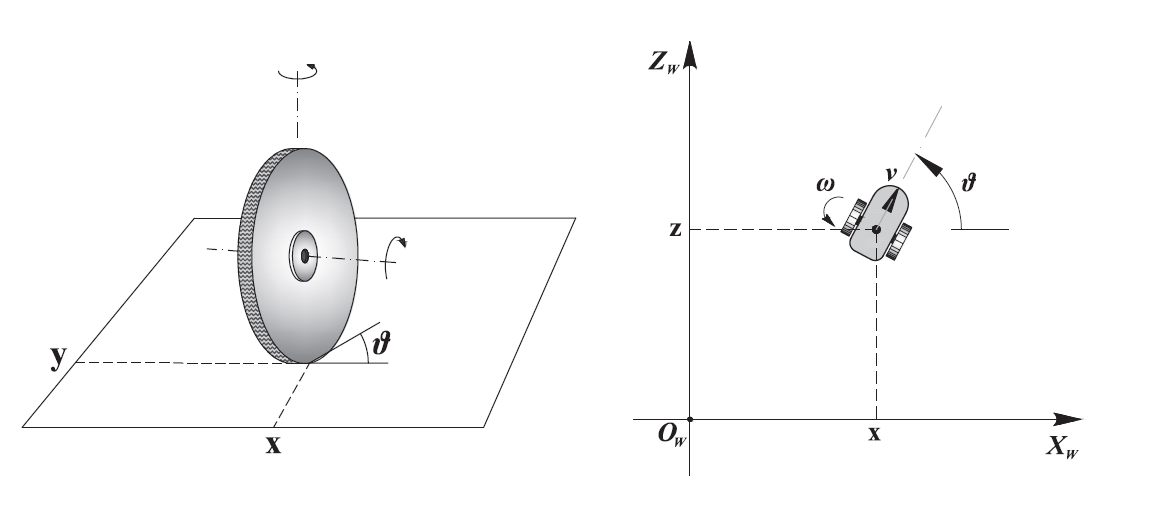
\includegraphics[width=0.6\textwidth]{figs/Uniciclo}
\caption[The Unicycle Model]{The Unicycle Model.}
\end{center}
\end{figure}

From a purely control point of view, the problem of posture control (point-to-point motion) is a problem of stabilization of a point of equilibrium in the vehicle state space. The linearized system becomes not completely achievable when the reference vehicle is immobile $v = \omega = 0$, as happens if we want to reach a constant position and orientation. This requires that posture stabilization should use intrinsically nonlinear control methods.

\subsection {Orientation Error}
The state feedback control law allows to calculate the orientation error, which is then integrated. In order to calculate accurately and avoid incorrect orientations we used the arctan2 function. The arctan2 function is a function that generates the angle within the four quadrants of the plane. It also allows to determine the sign and the right quadrant within which the angle is positioned within a range of $(-\Pi,\Pi]$.

\subsection {Problem set-up}
The K-Junior is of the differential type, i.e. it has two controllable wheels, which allow both linear and angular movement: in the first case the speeds of the two wheels are equal and the angular velocity is zero, while in the second, the wheel speed must be different. In particular, the vehicle turns anticlockwise, if the speed of the left wheel is a negative sign and that of the right wheel is positive, and vice versa.\\
\\
Now let's see the parameters and the variables involved:\\
\begin{itemize}
\item ($x_{init}$, $y_{init}$) = initial position;
\item (x, y) = current position;
\item ($x_{des}$, $y_{des}$) = desired position;
\item V = costant linear velocity of the robot;
\item $\omega$ = angular velocity, calculated by the state feedback law;
\item $\vartheta$ = diretional angle in relation to the robot reference system;
\item $\vartheta_{des}$ = desired diretional angle, in order to reach the goal;
\item $\vartheta_{current}$ = diretional angle, to which the robot is directed;
\item $\vartheta_{init}$ = initial direction angle;
\item K = gain in closed loop;
\item $V_l$ = left wheel speed;
\item $V_r$ = right wheel speed;
\item L = distance between the center of the two wheels;
\end{itemize}
\begin{figure}[!h]
\begin{center}
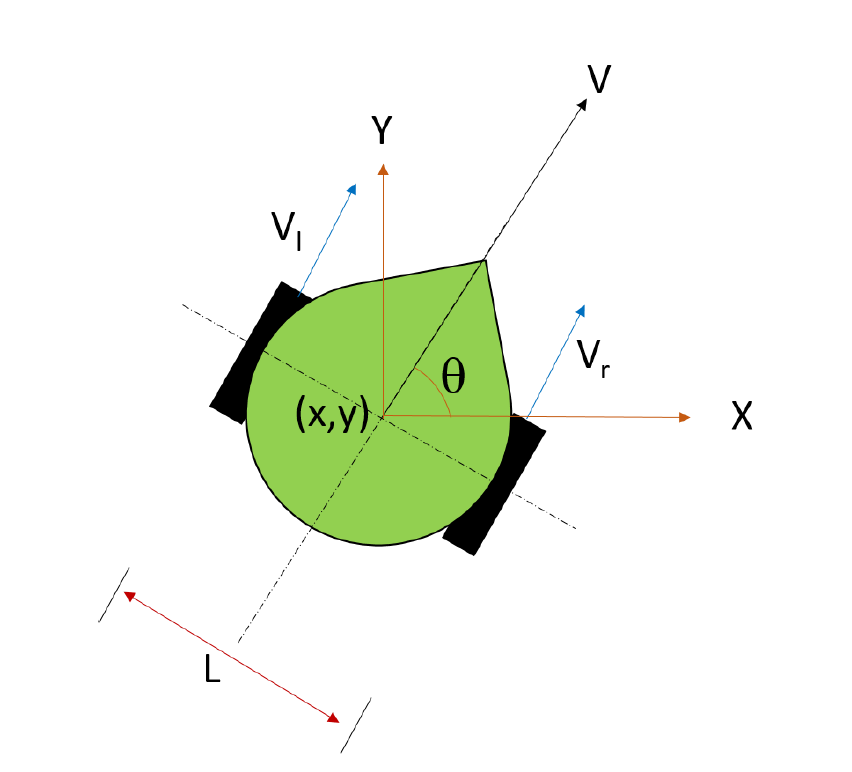
\includegraphics[width=0.8\textwidth]{figs/Robot}
\caption[Overview robot variables]{Overview robot variables.}
\end{center}
\end{figure}
The linear velocity V of the robot is given by the average of the individual speeds of the two wheels:
\begin{equation}
V=\frac{V_r + V_l}{2}
\end{equation}
During  modeling  of  the  robot  project,  we  made the following hypotheses:
\begin{itemize}
\item the robot moves at a costant speed;
\item the movement of the robot is evaluated for small time intervals; in this way $V_r$ and $V_l$, which are time-varying components, may be costant in such intervals; 
\item the wheels of the robot don't slip on the surface, compromising the speed of movement.
\end{itemize}

\subsection {Kinematic Equations}
The geometry of a moving body is rapresented by the three spatial coordinates and the temporal coordinates. The kinematic equations that evaluate the long displacement x and y are:
\begin{displaymath}
\dot{x} = V \cdot \cos{\vartheta}
\end{displaymath}
\begin{displaymath}
\dot{y} = V \cdot \sin{\vartheta}
\end{displaymath}
where $\vartheta$ is obtained from the integration of the angular speed of the robot:
\begin{displaymath}
\dot{\vartheta} = \omega = K \cdot (\vartheta_{des} - \vartheta_{current}) = K \cdot e
\end{displaymath}

The system is closed loop if we apply the previous state feedback law, in which $\omega$ is, along with constant V, the input of our system, while $\vartheta$ represents the state of the system. The difference $(\vartheta_{des} - \vartheta_{current})$ represents the error system $e$. So we are applying a feedback on the error system.

\section{Implemented solutions}
\subsection {Simulation}
\subsubsection{Description}
\begin{figure}[!h]
\begin{center}
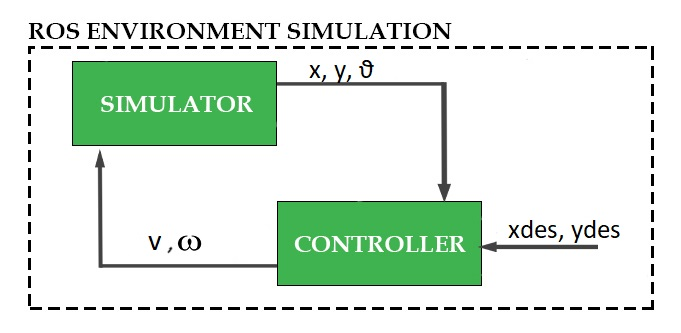
\includegraphics[width=0.8\textwidth]{figs/Simulation}
\caption[Simulation block diagram]{Simulation block diagram.}
\end{center}
\end{figure}

The simulation phase is implemented entirely using Python and it is developed using:
\begin{itemize}
\item two ROS nodes: Controller and Simulator
\item two communication topics: /input\textunderscore topic and /position\textunderscore topic
\item two message files: Input.msg and Position.msg
\end{itemize}

When the Simulator is started, the subscriber keeps listening on the /input\textunderscore topic until the Controller publishes the linear speed, which is constant in our case, and the angular speed, which is computed using a control law. At first, the Controller takes from input the desired destination coordinates ($x_{des}, y_{des}$) and it takes care of the computation of:
\begin{itemize}
\item the distance
\begin{equation} 
dis = \sqrt{(x_{des} - x)^{2} + (y_{des} - y)^{2}} 
\end{equation}
\item the desired orientation angle 
\begin{equation}
\vartheta_{des} = arctan(\dfrac{y_{des} - y}{x_{des} - x})
\end{equation}
\item the angular speed
\begin{equation}
\omega = K(\vartheta_{des} - \vartheta_{current})
\end{equation}
\end{itemize}
		
where x, y, and $\vartheta$ represent the current position of the robot. At the first iteration, they correspond to the constant variables $x_{init}  = 0$, $y_{init}  = 0$, $\vartheta_{init}  = 0$. Then, the computed $\vartheta_{des}$ is subjected to control in order to bound it in a [-180$^{\circ}$, 180$^{\circ}$] range. The calculated angular speed is controlled as well, bounding it in a [-1, 1] range, because of what we know about the unicycle theory, as seen in \cite{MR-GB:55}. So, the Controller publishes the linear speed (constant at 0.16) and the angular speed on the $/input\textunderscore topic$. The Simulator subscribes the speeds and deals with the computation of the current position and angle using the integration of movement dynamics:
$$\vartheta = \int_{t}^{t+\Delta t} \dot{\vartheta} \> dt = \int_{t}^{t+\Delta t} \omega \> dt $$\\
$$x = \int_{t}^{t+\Delta t} \dot{x} \> dt = \int_{t}^{t+\Delta t} v \> cos(\vartheta) dt $$\\
$$y = \int_{t}^{t+\Delta t} \dot{y} \> dt = \int_{t}^{t+\Delta t} v \> sin(\vartheta) dt $$\\

where the time range $\Delta t$ is calculated on a frequency of 100 Hz, corresponding to 0,01 seconds. Afterwards, the Simulator publishes x, y, and $\vartheta$ on the $/position\textunderscore topic$, so they can be subscribed by the Controller. In fact, after the Controller receives the data about the current position and orientation of the robot, it calculates again the distance, the desired diretional angle $\vartheta$ and the angular speed $\omega$. At this point, a distance check is made between the current position and the destination (entered at the beginning).\\
\\
\\If the distance is:
\begin{itemize}
\item less than a certain quantity $dist\textunderscore des$ (constant at 0.1), the linear speed is set to 0 and the simulation terminates, because the destination is reached;
\item less than a certain quantity $dist\textunderscore near$ (constant at 0.5), the linear speed is halved and set to 0.08. In this way, the vehicle can slow down near the destination;
\item otherwise, the linear speed remains unchanged at 0.16 and the simulation continues.
\end{itemize}

The procedure is repeated with the publication of the linear and angular speeds on the /input\textunderscore topic and the simulation is iterated until the target is reached. This loop is guided by the above mentioned distance check that we find in the Controller. At the end of the simulation when the destination is reached, the Controller produces two plots: the first one is related to the movement in the xy plane and it represents a sequence of points corresponding to the positions taken by the robot. An arrow is placed on each point, representing the orientation angle; the second plot shows the variation of the angular speed $\omega(t)$ with respect to time. The position (x, y) and the orientation $\vartheta$ are stored in a log.txt file at each iteration.

\subsubsection{PSEUDOCODE}
Below, the pseudocode of the nodes previously described.\\
CONTROLLER:
\begin{itemize}
\item insertion from input of ($x_{des}, y_{des}$)
\item computation of distance,  $\vartheta_{des}$ and angular speed
\begin{itemize}
\item control on $\vartheta_{des}$  and angular speed
\end{itemize}
\item publication of (v, $\omega$) on the $/input\textunderscore topic$
\item subscription to the $/position\textunderscore topic$ in order to read the (x, y, $\vartheta$) published by the Simulator
\item LOOP:
\begin{itemize}
\item distance check (dis):
\begin{itemize}
\item if $dis < dist\textunderscore des \rightarrow v = 0$ destination reached. Exit from the program;
\item if $dis < dist\textunderscore near \rightarrow v = 0.08$ the robot is near the destination;
\item else $v = 0.16$ the linear speed remains unchanged.
\end{itemize}
\item computation of  $\vartheta_{des}$ and angular speed
\begin{itemize}
\item control on  $\vartheta_{des}$  and angular speed
\end{itemize}
\item publication of (v, $\omega$) on the $/input\textunderscore topic$
\item subscription to the $/position\textunderscore topic$ in order to read the (x, y, $\vartheta$) published by the Simulator
\end{itemize}
\item generation of the final plots
\end{itemize}

SIMULATOR:
\begin{itemize}
\item subscription to the $/input\textunderscore topic$ in order to read the (v, $\omega$) published by the Controller
\item computation of $\dot{\vartheta}, \dot{x}, \dot{y}$
\item computation of x, y, $\vartheta$ using the integration with respect to time of $\dot{\vartheta}, \dot{x}, \dot{y}$
\item publication of (x, y, $\vartheta$) on the $/position\textunderscore topic$
\end{itemize}

\subsection {Experiment}
\subsubsection{Description}
\begin{figure}[H]
\begin{center}
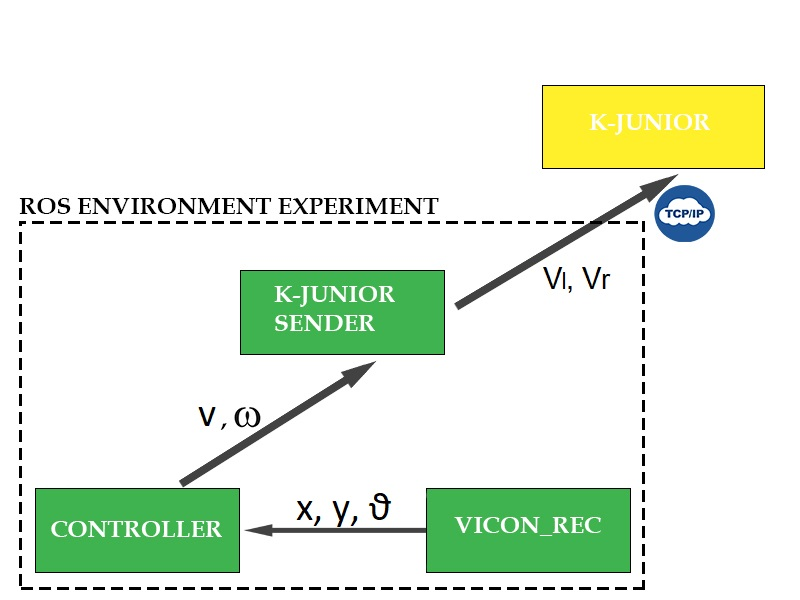
\includegraphics[width=0.8\textwidth]{figs/Experiment}
\caption[Experiment block diagram]{Experiment block diagram.}
\end{center}
\end{figure}

The experimentation phase is implemented using both Python and C/C++ and it is developed using:
\begin{itemize}
\item three ROS nodes: Controller, Receiver and Sender
\item one Server set on the robot
\item two communication topics: ViconTopic and SenderTopic
\item two message files: Input.msg and ViconMsg.msg
\end{itemize}
At first, the connection with the robot (IP address: 192.168.0.41) is established using the appropriate command and the Server is launched. It always keeps running waiting for the speeds of the wheels sent from the client, which is our Sender, in order to set the speed on the vehicle allowing it to move. This process is possible after the initialization of the kj-evo library, in order to have access to the methods dealing with the movement of the robot.
\\
At the same time and from another workstation, the connection with the infrared camera system is established. With a frequency of 100 Hz, this system captures the position of the robot and the rotation matrix associated to it. The data are received from the Receiver node and they are used in order to extract the necessary information to continue the experiment. In this case, the only necessary data are the K-Junior position (x, y) and its angulation $\vartheta$, i.e. the angle of rotation about the z axis. The Receiver publishes the data on the ViconTopic using the ViconMsg message type.
\\
The Controller takes from input the destination coordinates ($x_{des}, y_{des}$) and it handles the subscription on the ViconTopic, so that it can read the current x, y, $\vartheta$. Then, the distance between the current position and the target is computed with the formula (1.2), in order to make a check on it. If the distance is:
\begin{itemize}
\item less than a certain quantity $dist\textunderscore des$ (constant at 0.1), the linear speed is set to 0 and the experiment terminates, because the destination is reached;
\item otherwise, the linear speed remains unchanged at 0.112.
\end{itemize}
Afterwards, the desired diretional angle $\vartheta_{des}$ and the angular speed $\omega$ are computed, using the formulas (1.3) and (1.4). The computed  $\vartheta_{des}$ is subjected to control in order to bound it in a [-180$^{\circ}$, 180$^{\circ}$] range.
At last, the Controller publishes the (v, $\omega$) on the SenderTopic using the Input message type.
\\ At this point the Sender, which is the Client TCP, connects to the Server that is running on the robot. Once the connection is established, the Sender subscribes on the SenderTopic and reads the linear and angular speeds published by the Controller. A check on the linear speed is executed: in fact, if it is equal to zero, a message is sent to the Server to notify the stop of the wheels. When the linear speed is not equal to zero, a check on the angular speed is performed in order to bound it in a [-1, 1] range, just like the unicycle model imposes, as seen in \cite{MR-GB:55}.
\\ Afterwards, the Sender executes a mapping of the wheels speeds, according to the value of the angular speed, explained later in this chapter. These velocities are concatenated into a String and then sent to the Server via socket.
\\ The Server receives the data from the Client as a String variable and then converts it into two Integer values. Then, the wheels speeds are set to the motors of the robot using the appropriate method.
\\ Once the robot performs the movement, the cycle starts again and the Receiver captures the current position of the robot using the cameras system.
\\ The Controller stores the position (x, y) and the orientation $\vartheta$ in a  $log\textunderscore vicon.txt$ file at each iteration, until the destination is reached.

\subsubsection{PSEUDOCODE}
Below, the pseudocode of the nodes previously described.\\

RECEIVER:
\begin{itemize}
\item insertion of the Robot name in order to start the data reception
\item creation of the client
\item connection to the vicon server
\item LOOP:
\begin{itemize}
\item capture of the data about the current position and the rotation matrix
\item publication of (x, y, $cos(\vartheta)$) on the ViconTopic
\end{itemize}
\end{itemize}

CONTROLLER:

\begin{itemize}
\item insertion from input of ($x_{des}, y_{des}$)
\item subscription to the ViconTopic in order to read (x, y, $cos(\vartheta)$) published by the Receiver
\item conversion of (x, y) in millimeters
\item application of the inverse cosine formula to obtain $\vartheta$
\item LOOP:
\begin{itemize}
\item computation of the distance
\item distance check:
\begin{itemize}
\item if $dis < dist\textunderscore des \rightarrow$ target reached, the linear speed is set to 0
\item else $\rightarrow$ the linear speed remains unchanged
\begin{itemize}
\item computation of $\vartheta_{des}$ and angular speed
\item control on $\vartheta_{des}$
\end{itemize}
\item publication of (v, $\omega$) on the SenderTopic
\end{itemize}
\end{itemize}
\end{itemize}

SENDER:
\begin{itemize}
\item connection to the robot Server
\item LOOP:
\begin{itemize}
\item subscription to the SenderTopic in order to read (v, $\omega$) published by the Controller
\item control on the linear speed:
\begin{itemize}
\item if $v = 0 \rightarrow V_l = 0, V_r = 0$
\item else $ \rightarrow $ mapping of v and $\omega$ into $V_l$ and $V_r$
\end{itemize}
\item conversion into String of $V_l$ and $V_r$
\item sending of the String variable to the Server
\end{itemize}
\end{itemize}

SERVER:
\begin{itemize}
\item starting of the Server
\item LOOP:
\begin{itemize}
\item receiving of the String variable with the wheels speeds
\item splitting of the String variable into two Integer values $V_l$ and $V_r$
\item setting of the motors speeds
\end{itemize}
\end{itemize}

\subsubsection{Mapping}
The following schema of the mapping is implemented in order to maintain a constant value for the linear speed v. Firstly, we bounded the angular speed $\omega$ into a [ -1, 1 ] range and, for each value of $\omega$, the values of the motors speed are assigned. In particular, it has been implemented a nested if-else statement, which is better explained in the table below:
\begin{itemize}
\item if $-0.1 \leq \omega \leq 0.1 \rightarrow V_l = 14, V_r = 14$
\item else if $0.1 < \omega \leq 0.5 \rightarrow V_l = 11, V_r = 17$
\item else if $0.5 < \omega \leq 1 \rightarrow V_l = 8, V_r = 20$
\item else if $-0.5 \leq \omega < -0.1 \rightarrow V_l = 17, V_r = 11$
\item else if $-1 \leq \omega < -0.5 \rightarrow V_l = 20, V_r = 8$
\end{itemize}
where $V_l$ and $V_r$ are respectively the speeds of the left wheel and the right wheel of the vehicle.
Each case developed in the if-else statement is associated to a linear speed of 11.2 cm/s. This value is computed using the linear speed formula (1.1).
From the documentation \cite{MR-GB:44}, we know that the maximum speed of the robot is 16 cm/s, so the input linear speed of the implemented system is sligthly less than the maximum possible value, but still constant.

%%%%%%%%% CAPITOLO  %%%%%%%%%%%%%%%%
\chapter{Results}
\section{Simulations results}
Below, it is shown how the course of the point changes when varying K for each simulation. The initial position is (0, 0) and the input destination given in order to perform the following simulations is (-3, -7). The project and the corresponding experiments are developed with a value of gain K which is equal to 1. In this section, different scenarios are explored, with a constant frequency of 100 Hz, integration interval $\Delta t = 0.01 s$ and a tolerance of 0.1. The linear speed is equal to 0.16 m/s, which is the maximum value of speed of the real vehicle, and it becomes 0.08 m/s when the distance from the destination point is less than 0.5. When the distance reaches a value which is less than the tolerance 0.1, the linear speed is set equal to 0 and the target is considered reached, so the simulation stops.

\begin{figure}[H]
\centering
\hspace*{-2.3in}
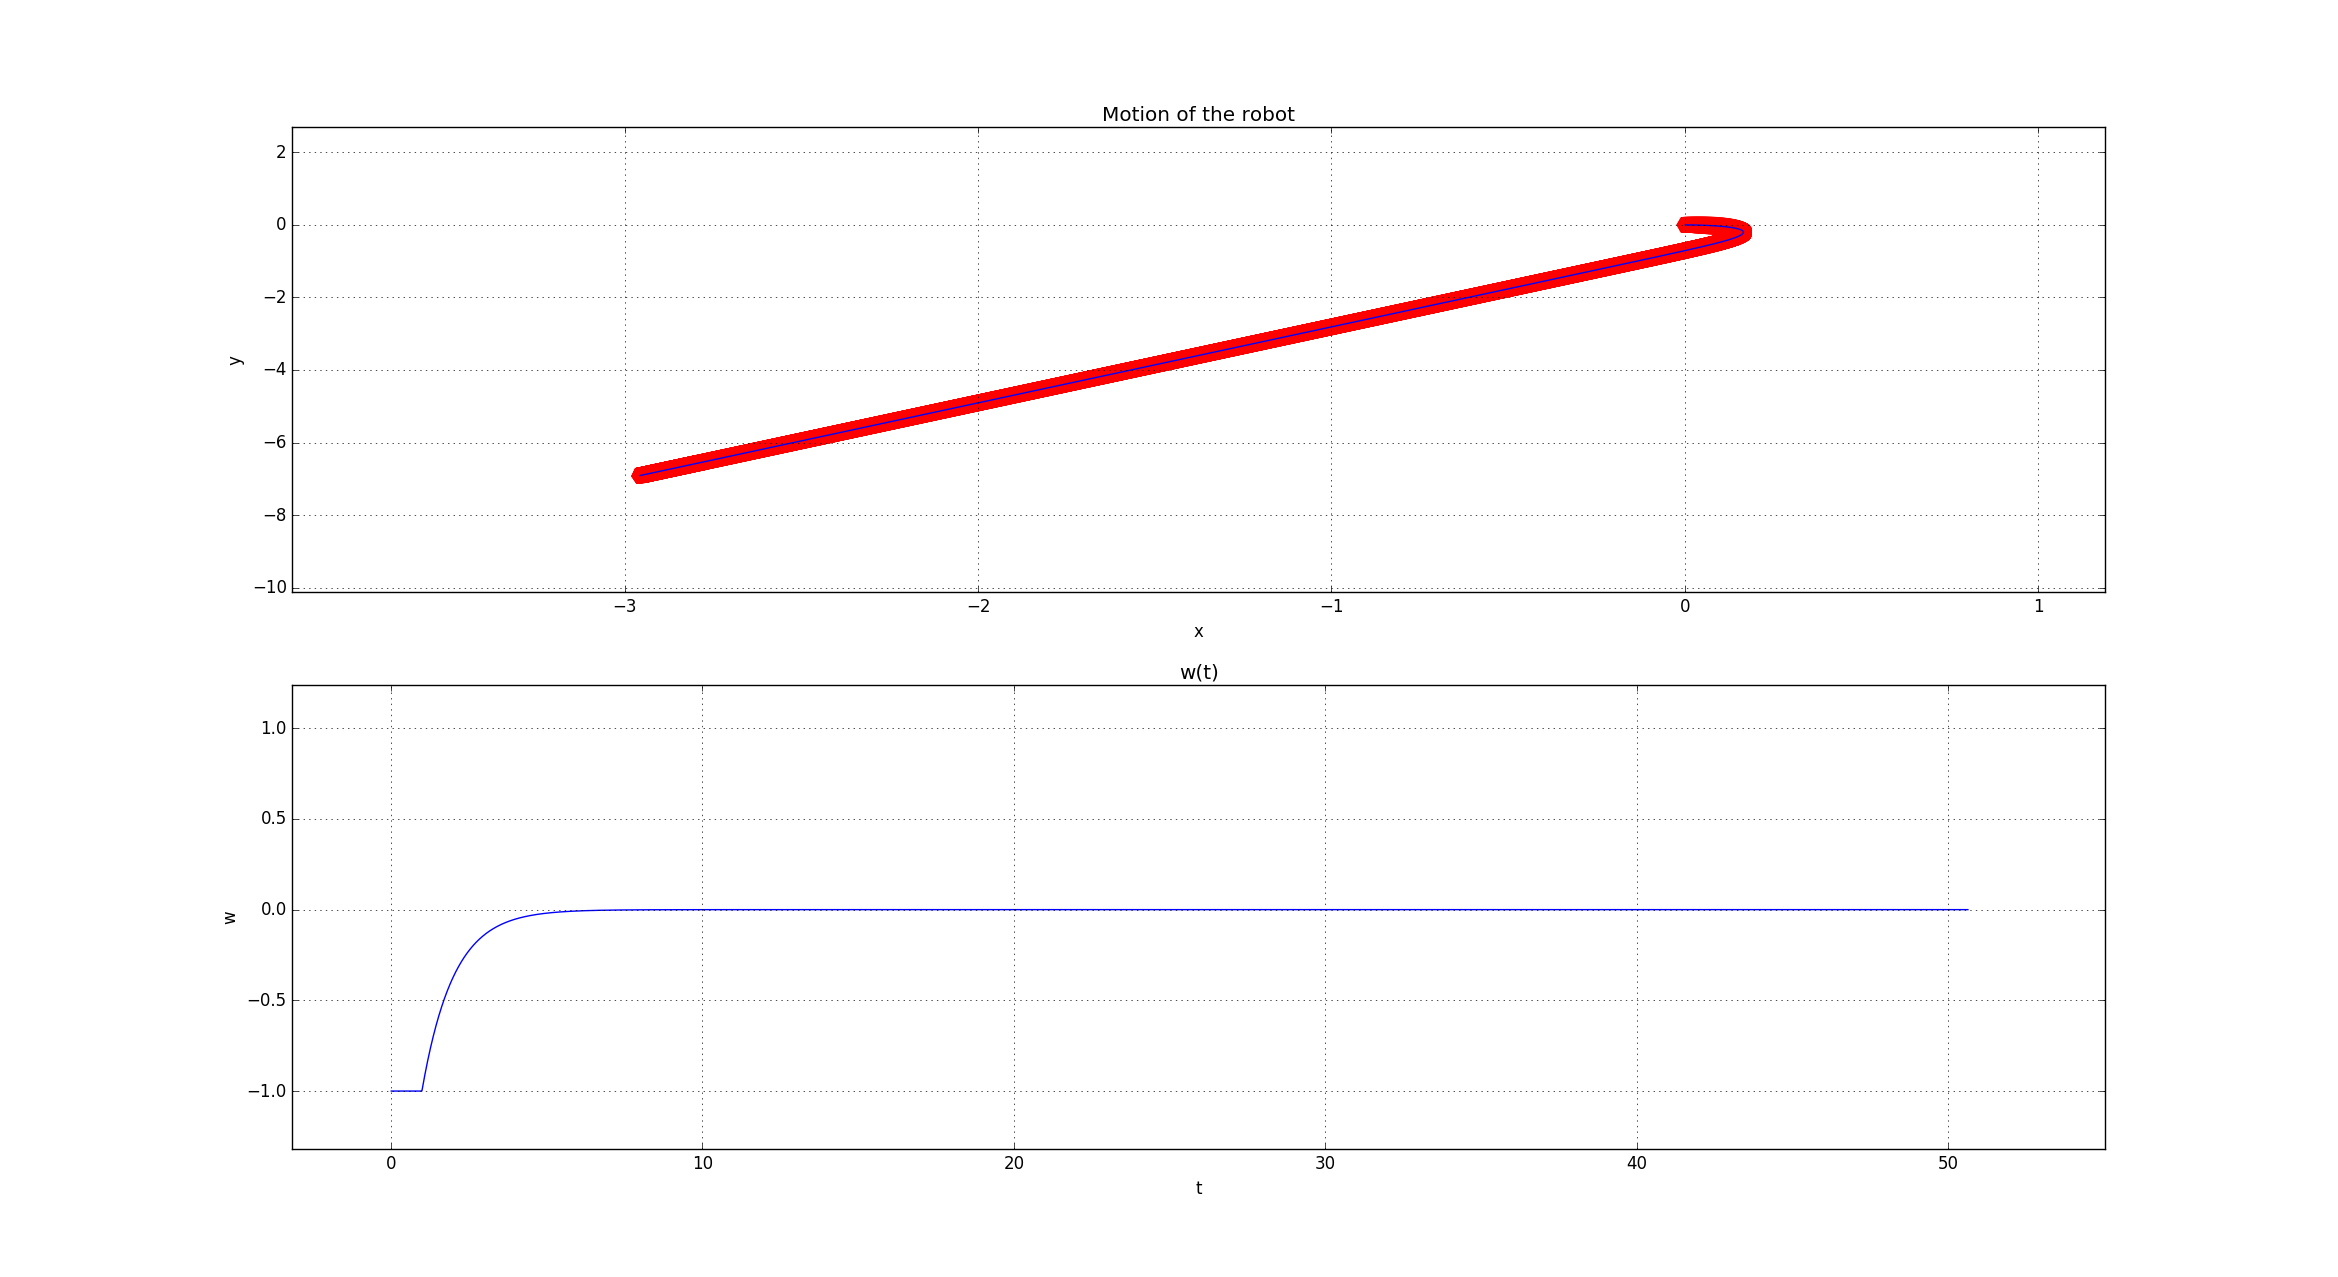
\includegraphics[width=1.9\textwidth]{figs/simulations/1_2}
\caption[Simulation: K = 1]{In this case, K is equal to 1 and it can be seen as the basic scenario that the next ones are compared to.}
\end{figure}

\begin{figure}[H]
\centering
\hspace*{-1.5in}
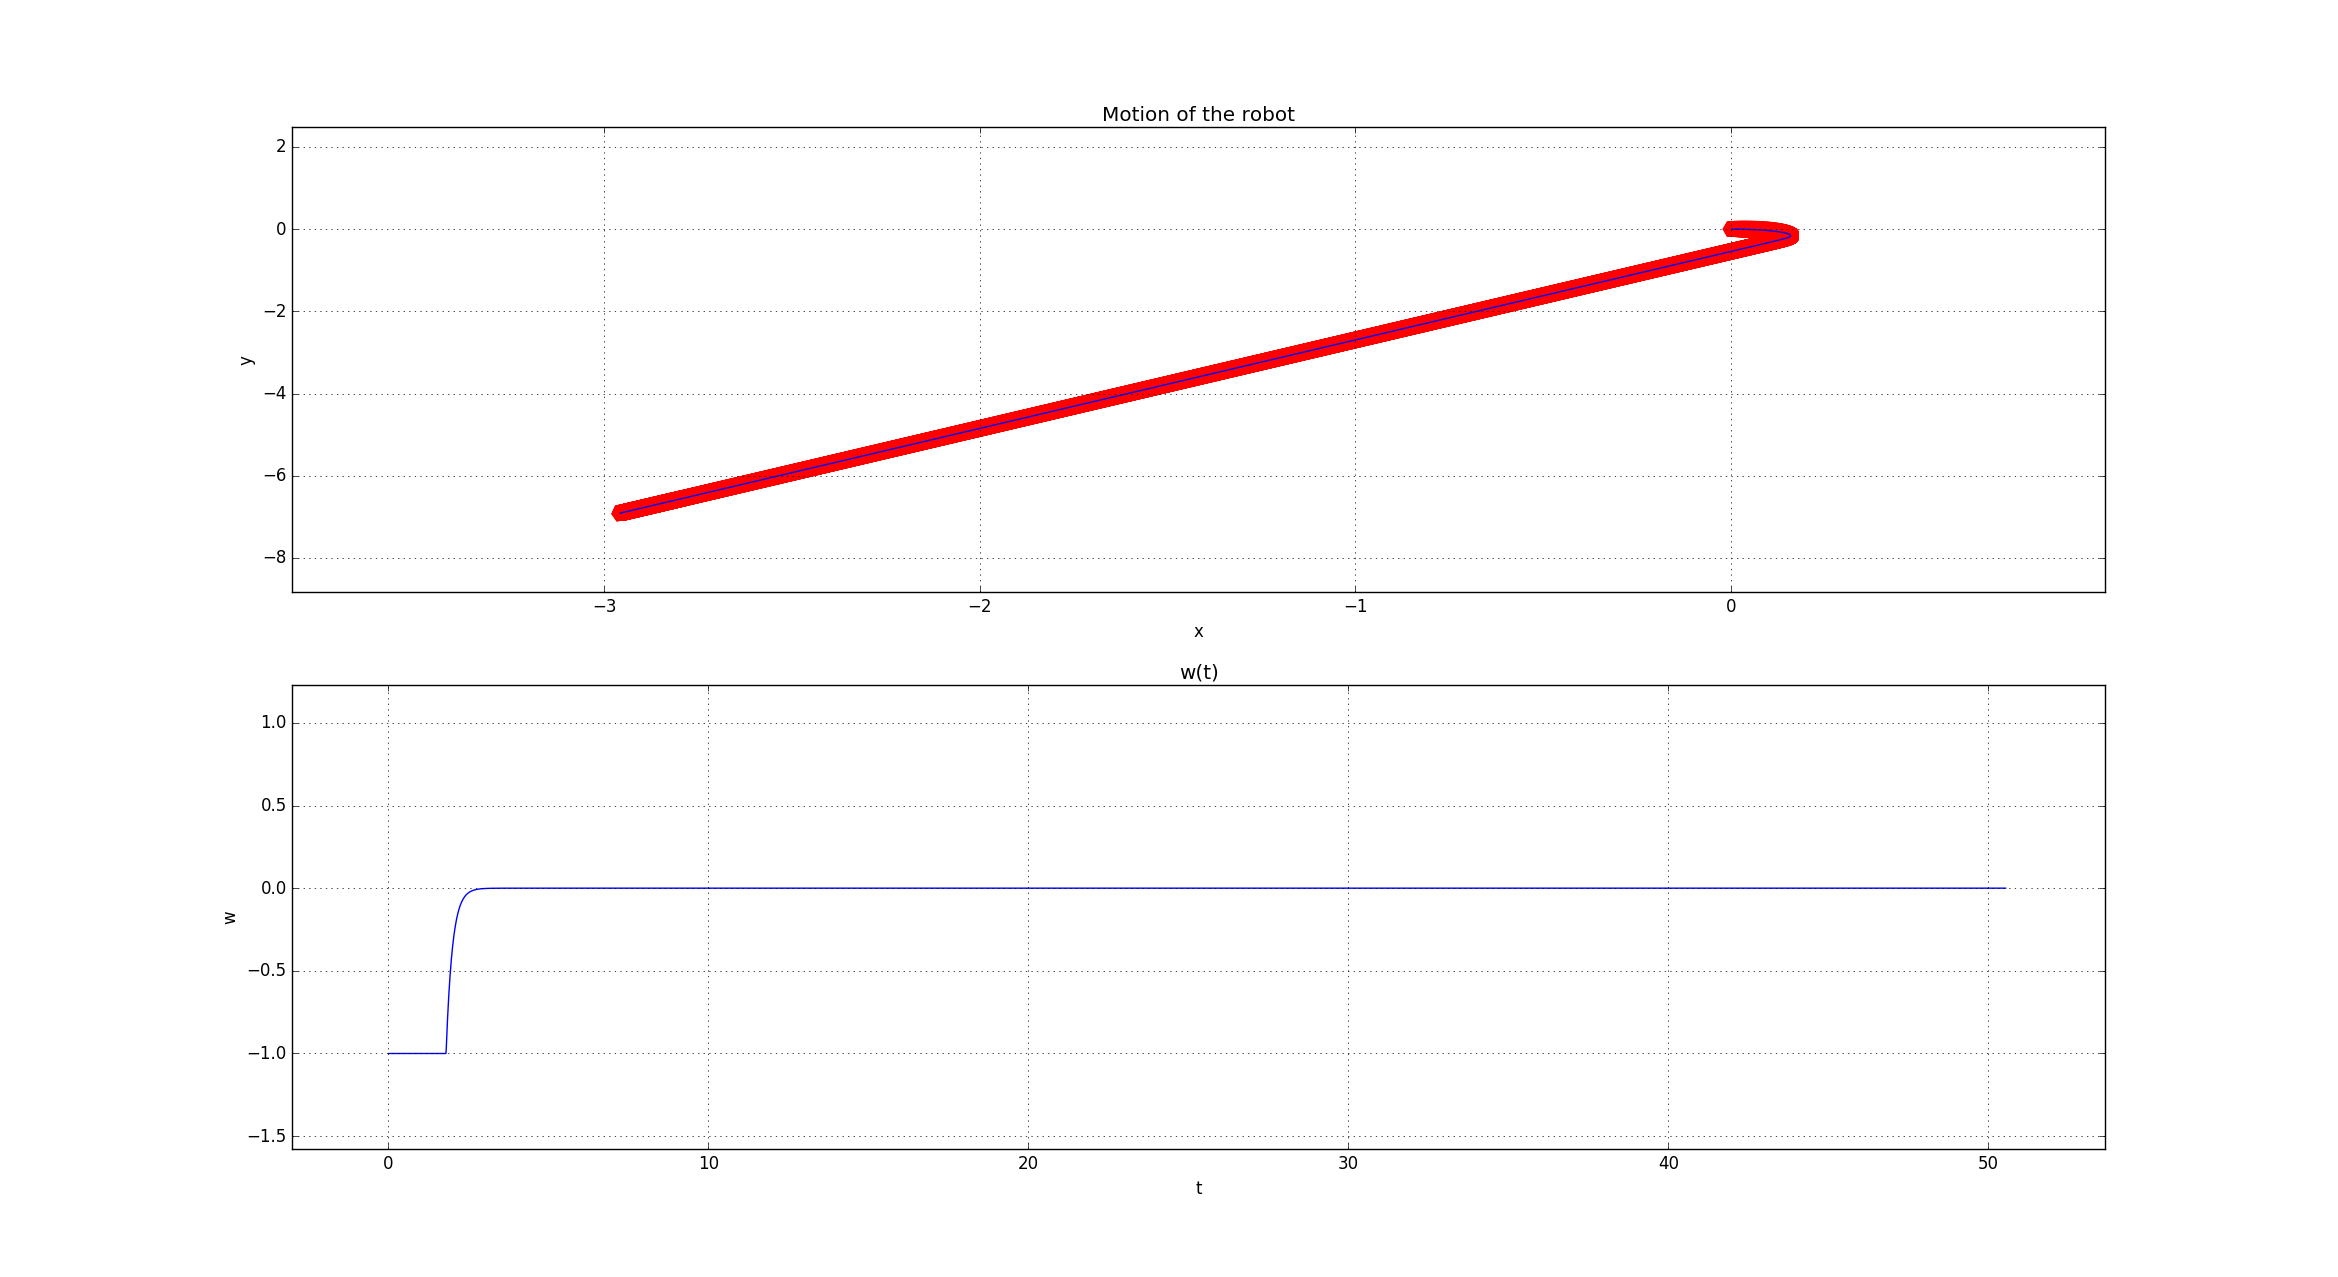
\includegraphics[width=1.5\textwidth]{figs/simulations/2_2}%
\qquad\qquad
\hspace*{-1.5in}
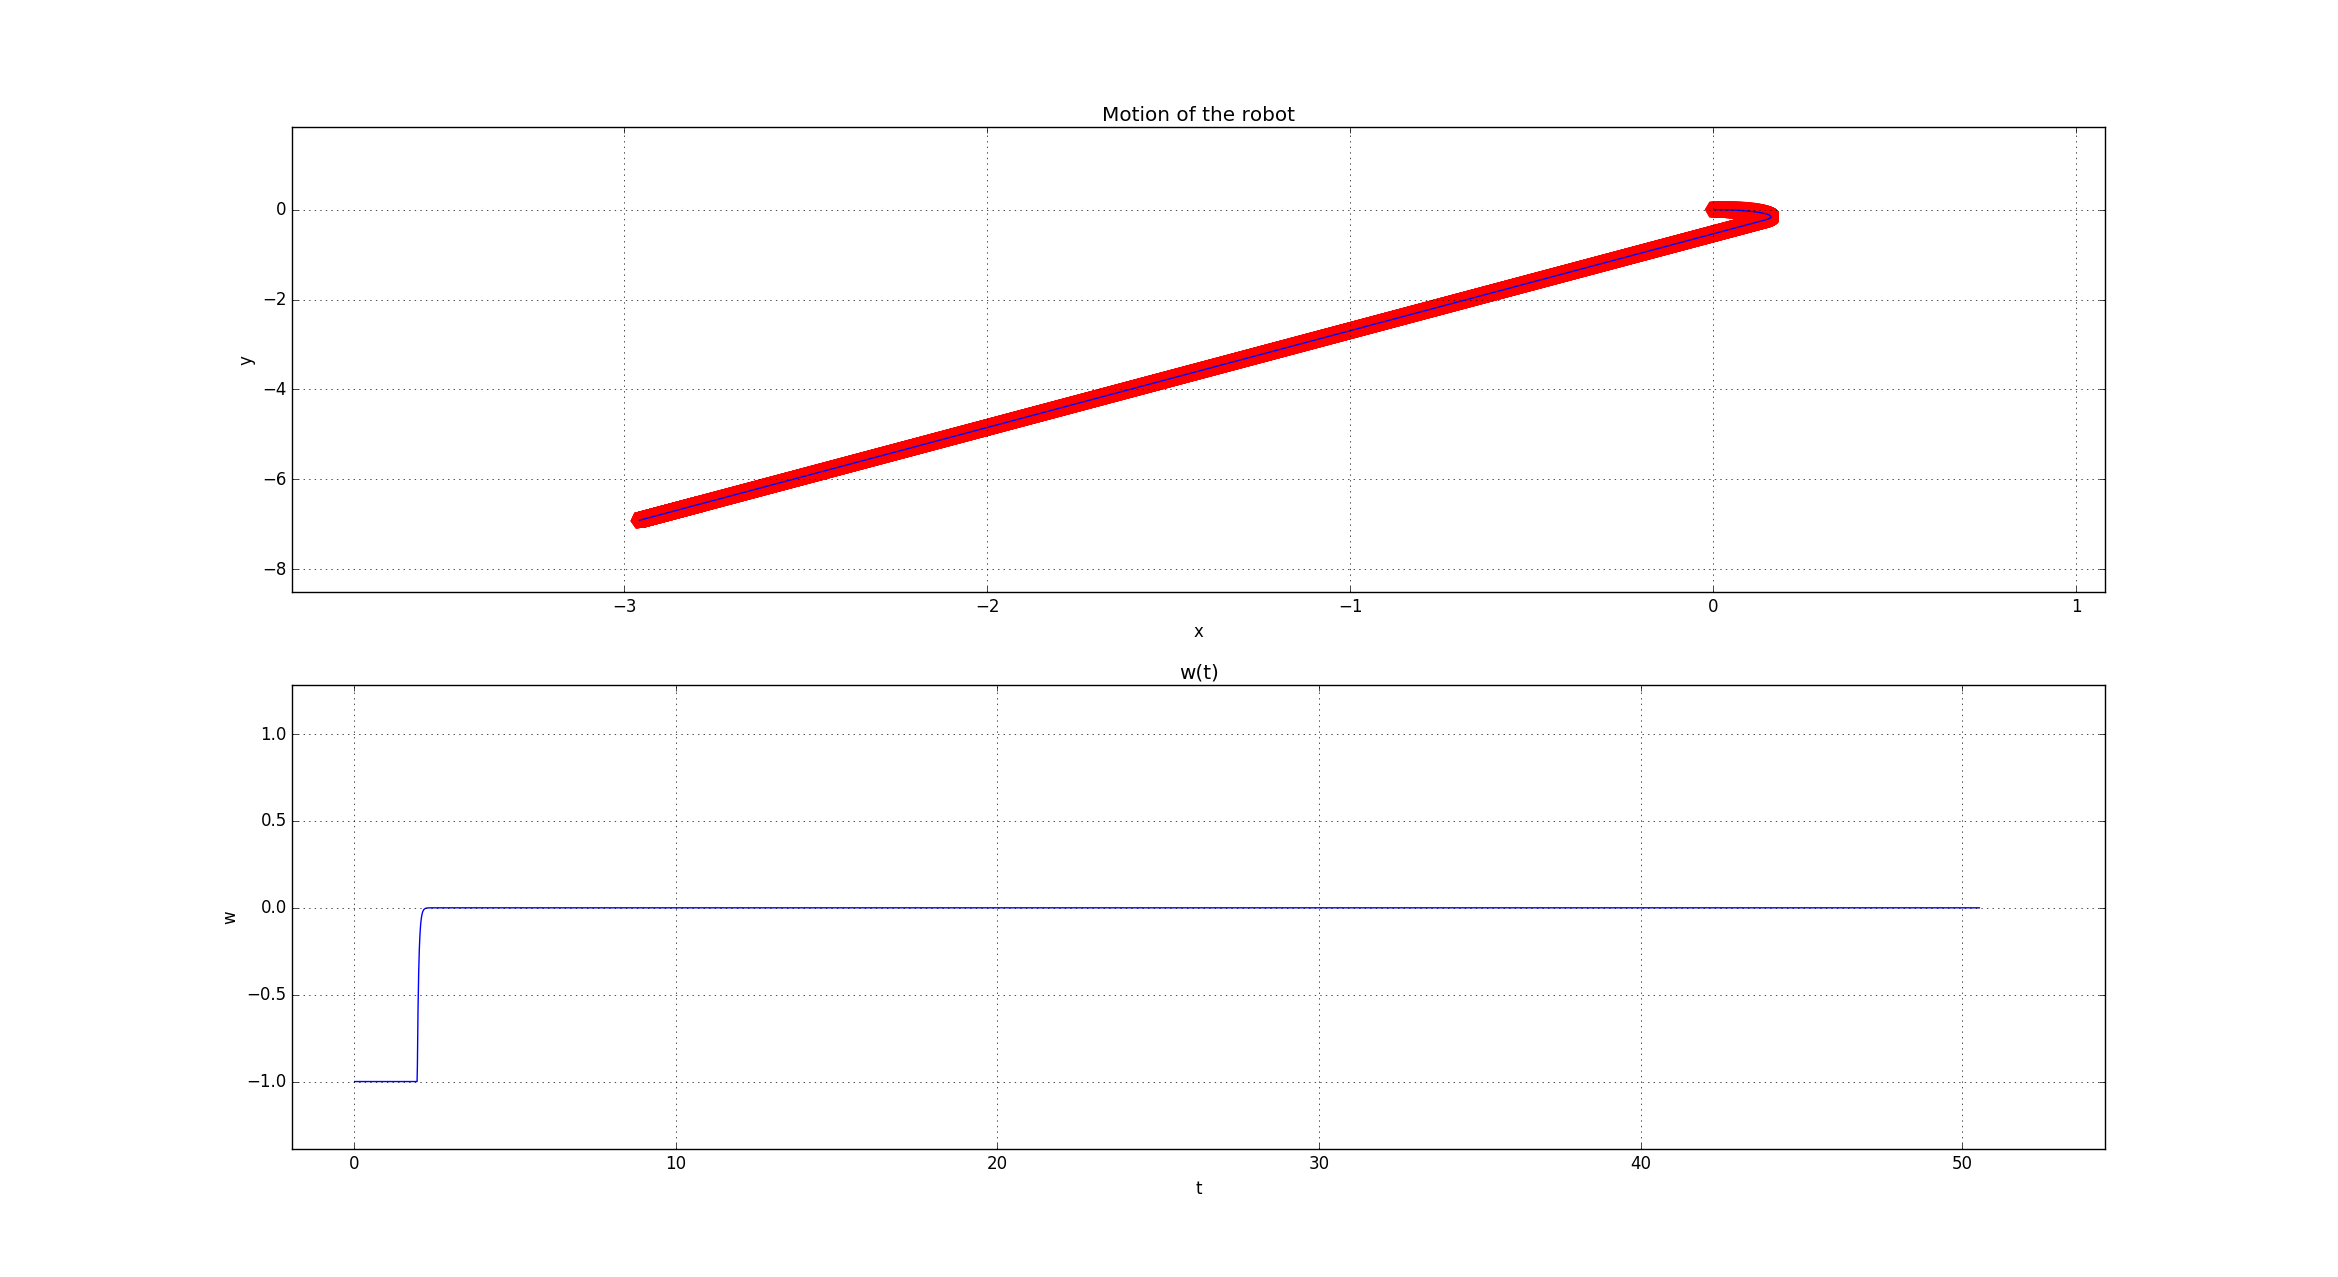
\includegraphics[width=1.5\textwidth]{figs/simulations/5_2}
\caption[Simulation: K = 5, K = 20]{These are both simulations for which the value K is greater than 1. In the first one is equal to 5, in the second it is equal to 20. As we can see in the plot regarding the variation of $\omega$ with respect to time, the slope is steeper for higher values of K. It tends to turn to the right trajectory in less time.}
\end{figure}

\begin{figure}[H]
\centering
\hspace*{-2.3in}
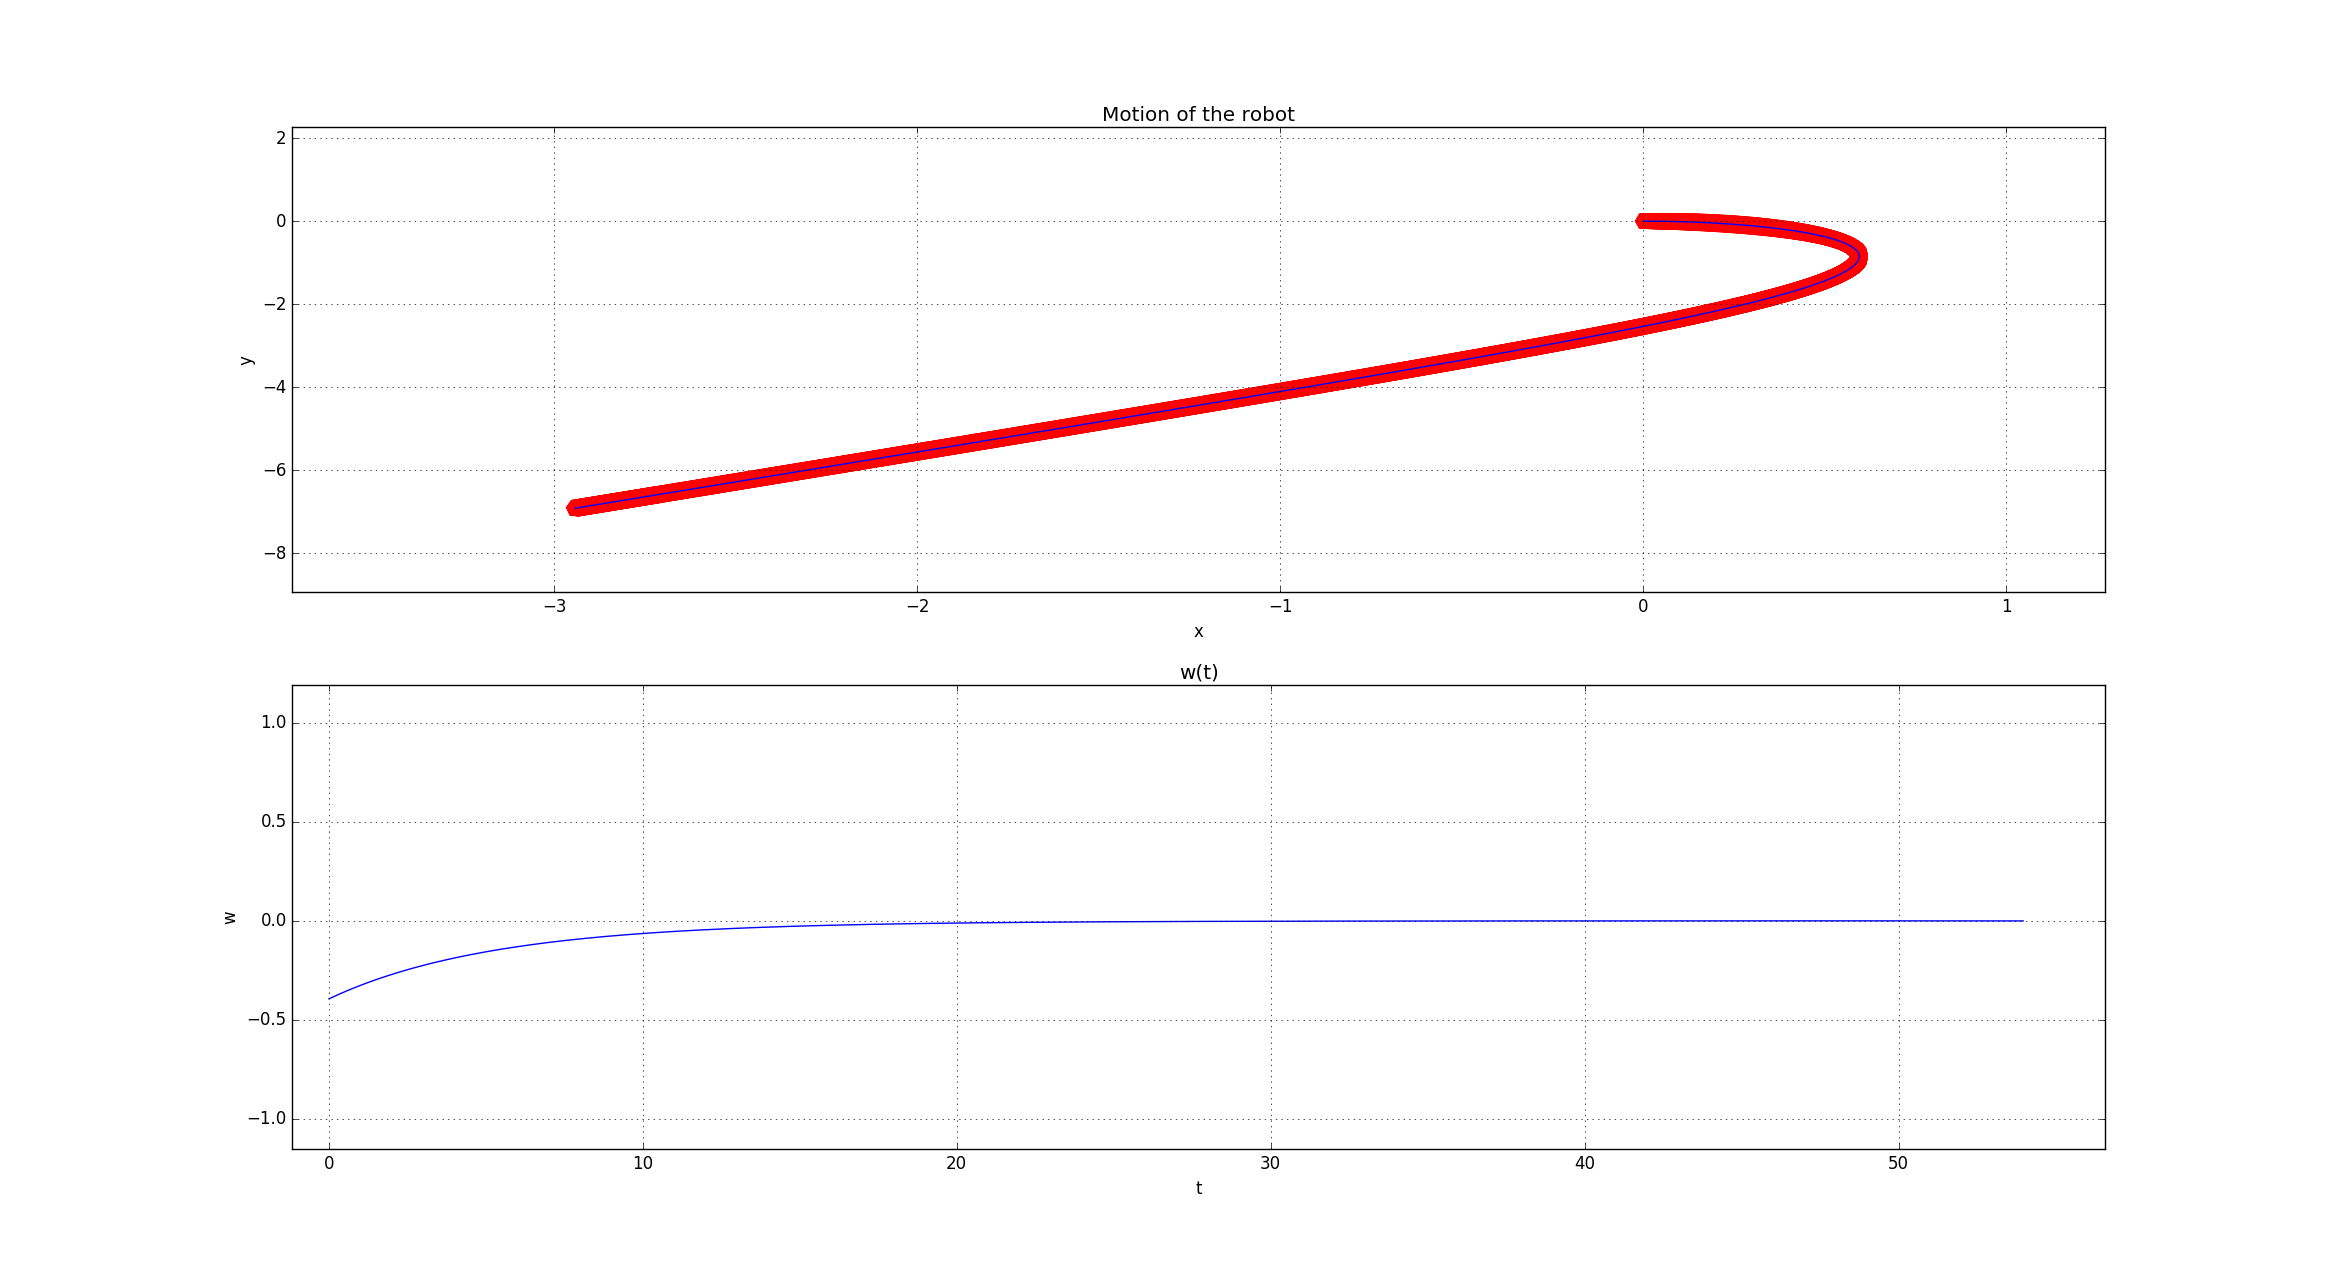
\includegraphics[width=1.9\textwidth]{figs/simulations/6_2}
\caption[Simulation: K = 0.2]{In this case, the value of K is bounded into a [0, 1] range, in fact it is equal to 0.2. Regarding to $\omega$, we see that the slope is way less steep than before, which means that the point takes more time to find the right trajectory, before going straight to it.}
\end{figure}

\begin{figure}[H]
\centering
\hspace*{-2.3in}
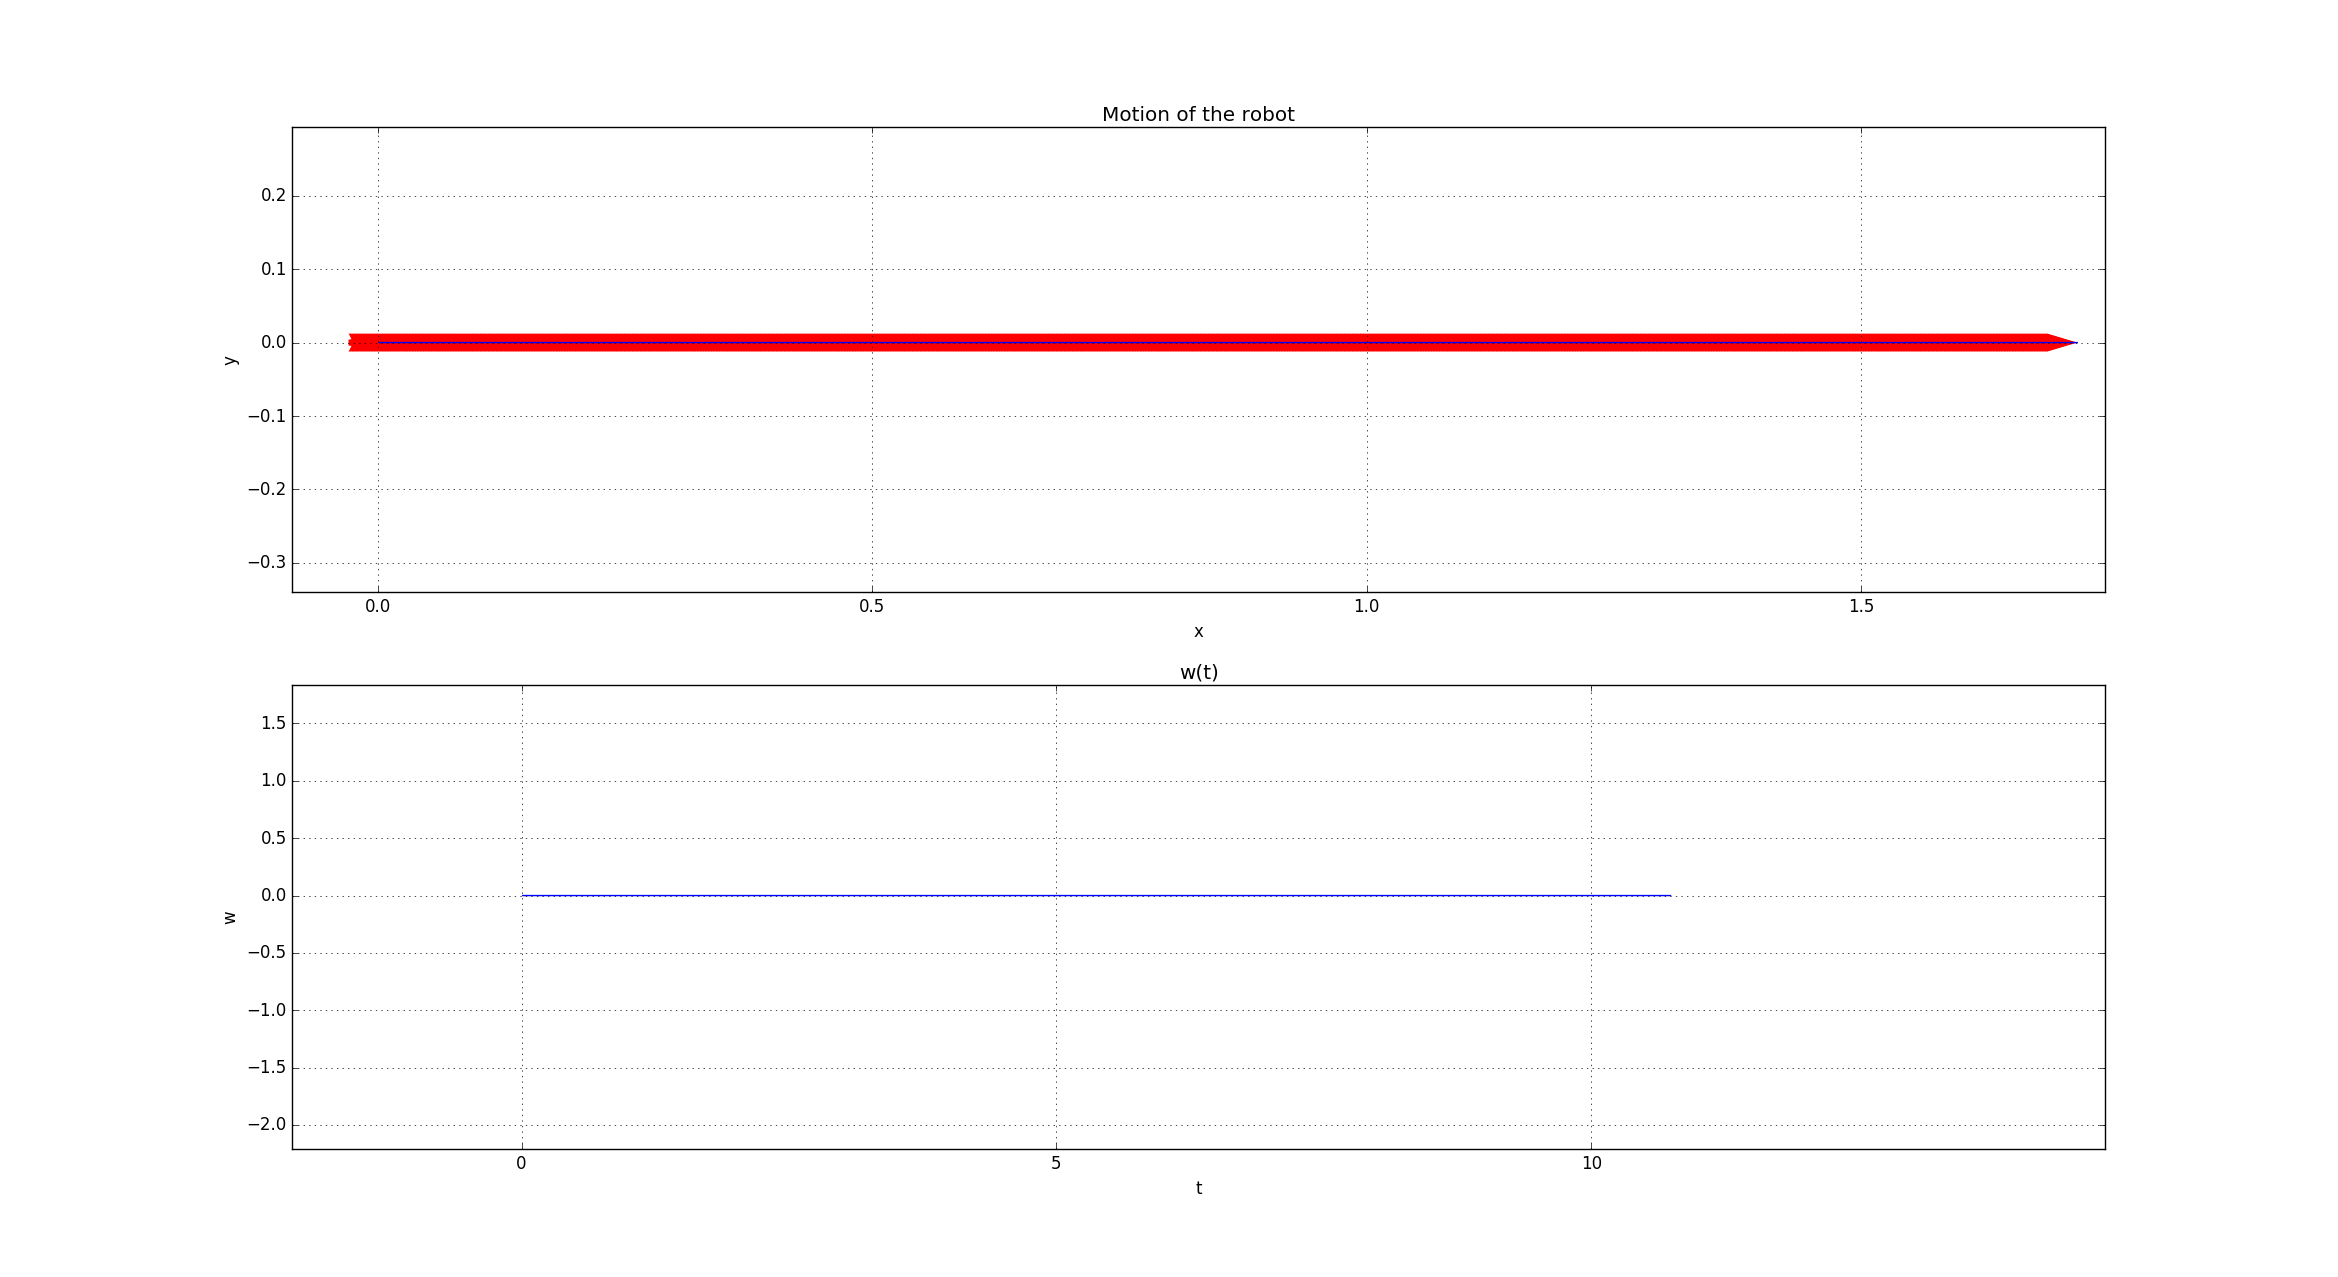
\includegraphics[width=1.9\textwidth]{figs/simulations/4_2}
\caption[Simulation: K = 0]{This is the case in which K is equal to 0, which means that we have no variation of $\omega$ with respect to time and the point goes straight until we force the stop of the simulation.}
\end{figure}

\begin{figure}[H]
\centering
\hspace*{-2.3in}
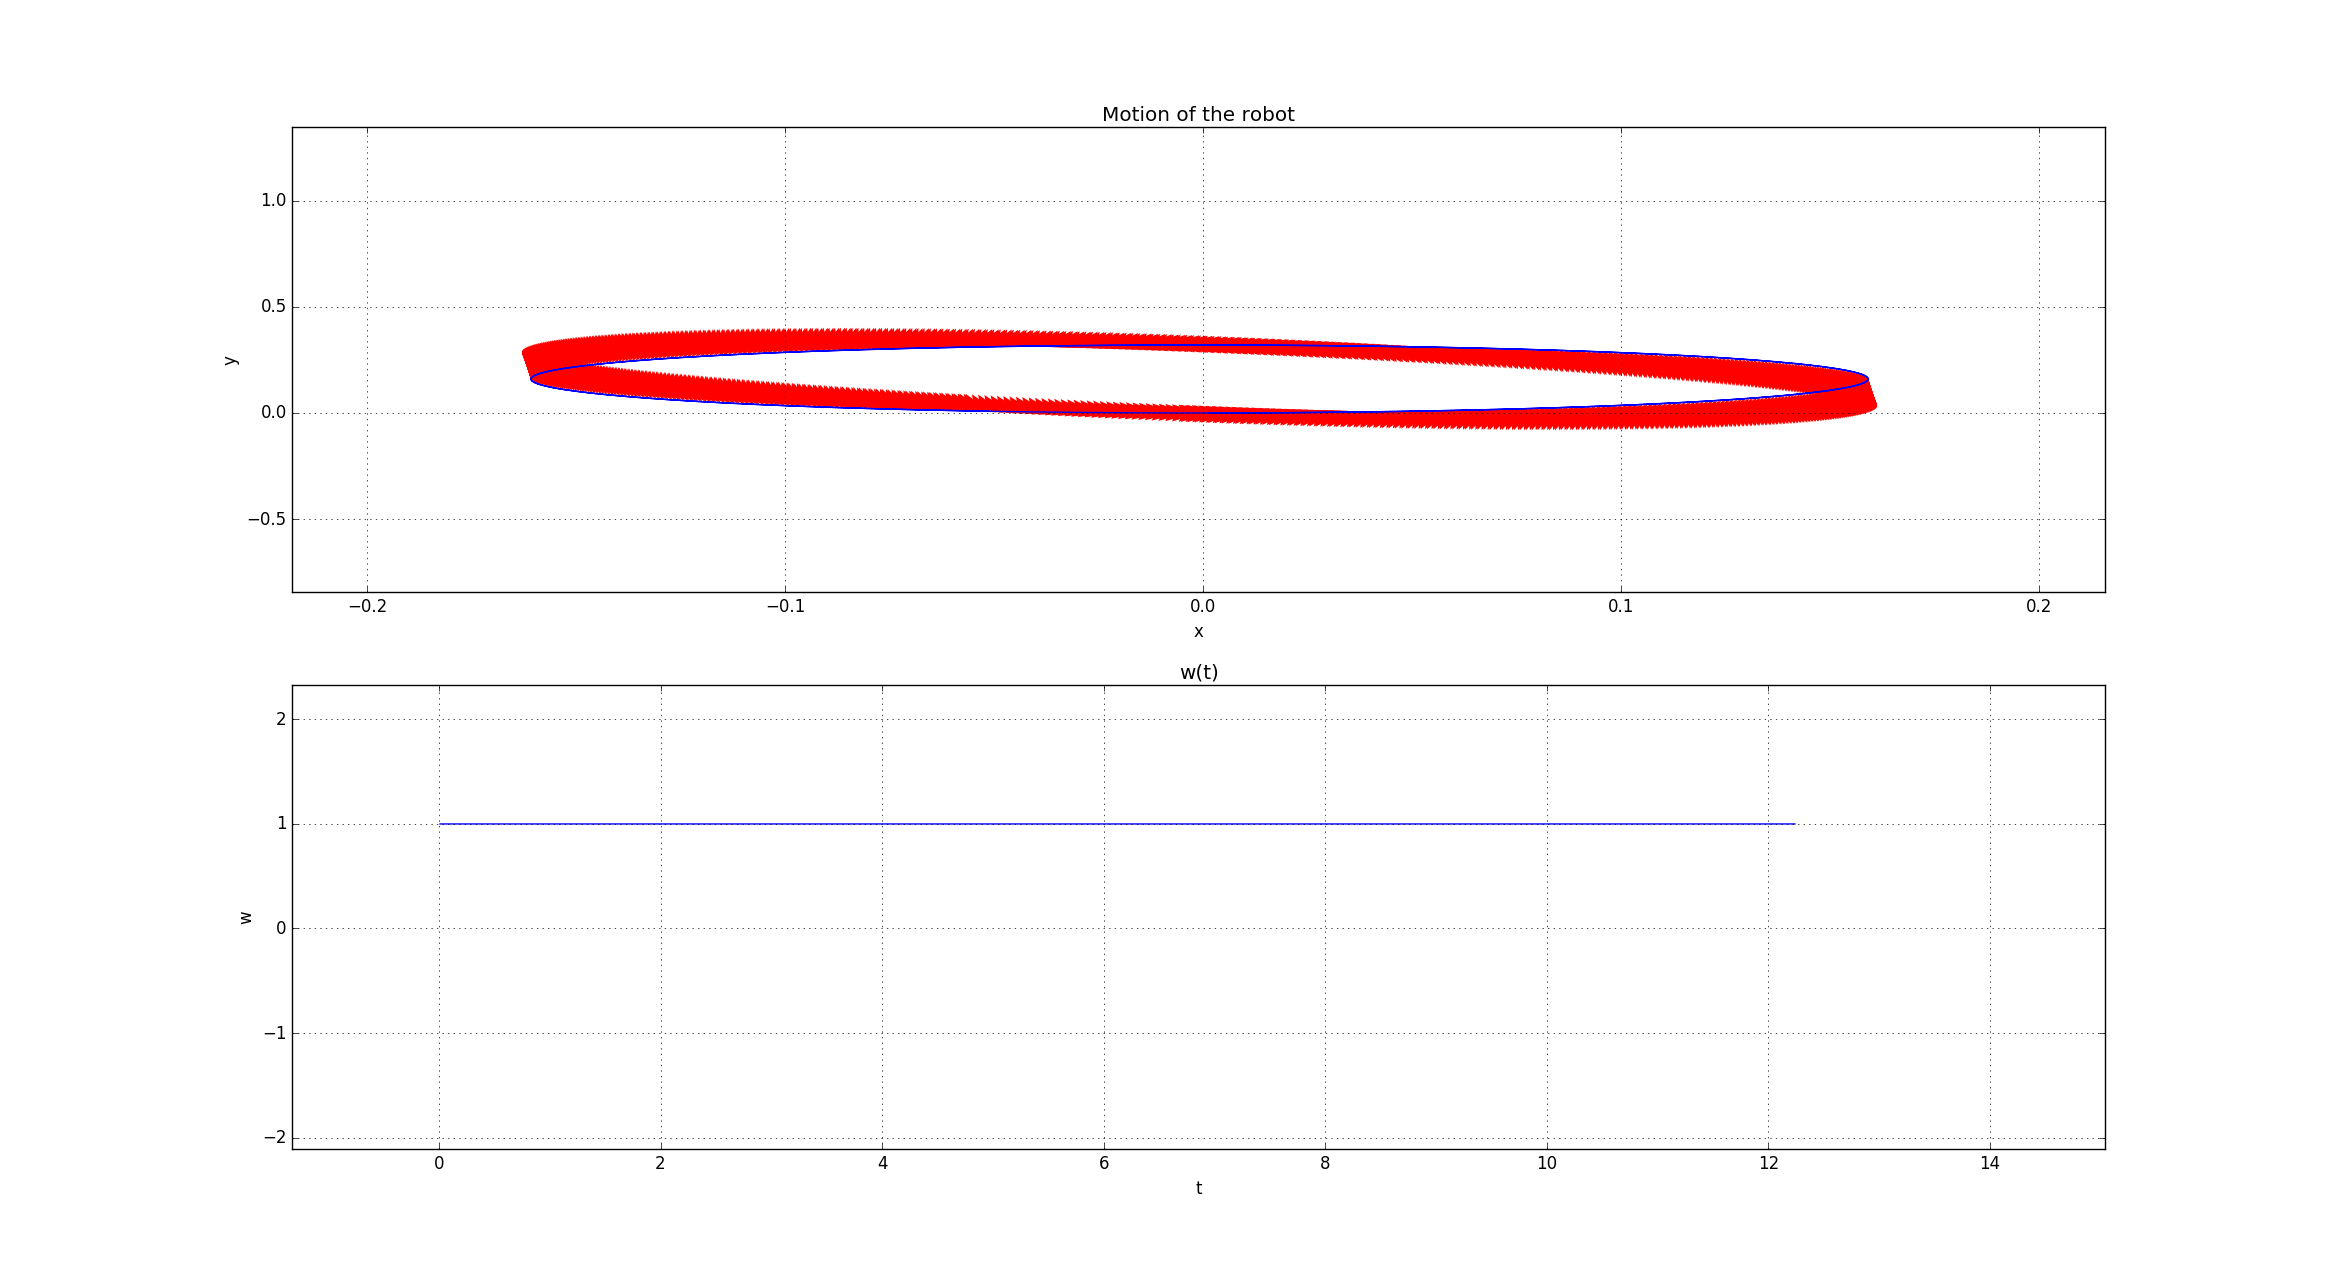
\includegraphics[width=1.9\textwidth]{figs/simulations/3_2}
\caption[Simulation: K = -1]{This is the final case taken into consideration and it is about the values of gain that are less than 0. In this specific plot, K is equal to -1. The point keeps spinning around itself and the value of $\omega$ remains constant to 1.}
\end{figure}

\begin{figure}[H]
\centering
\hspace*{-2.3in}
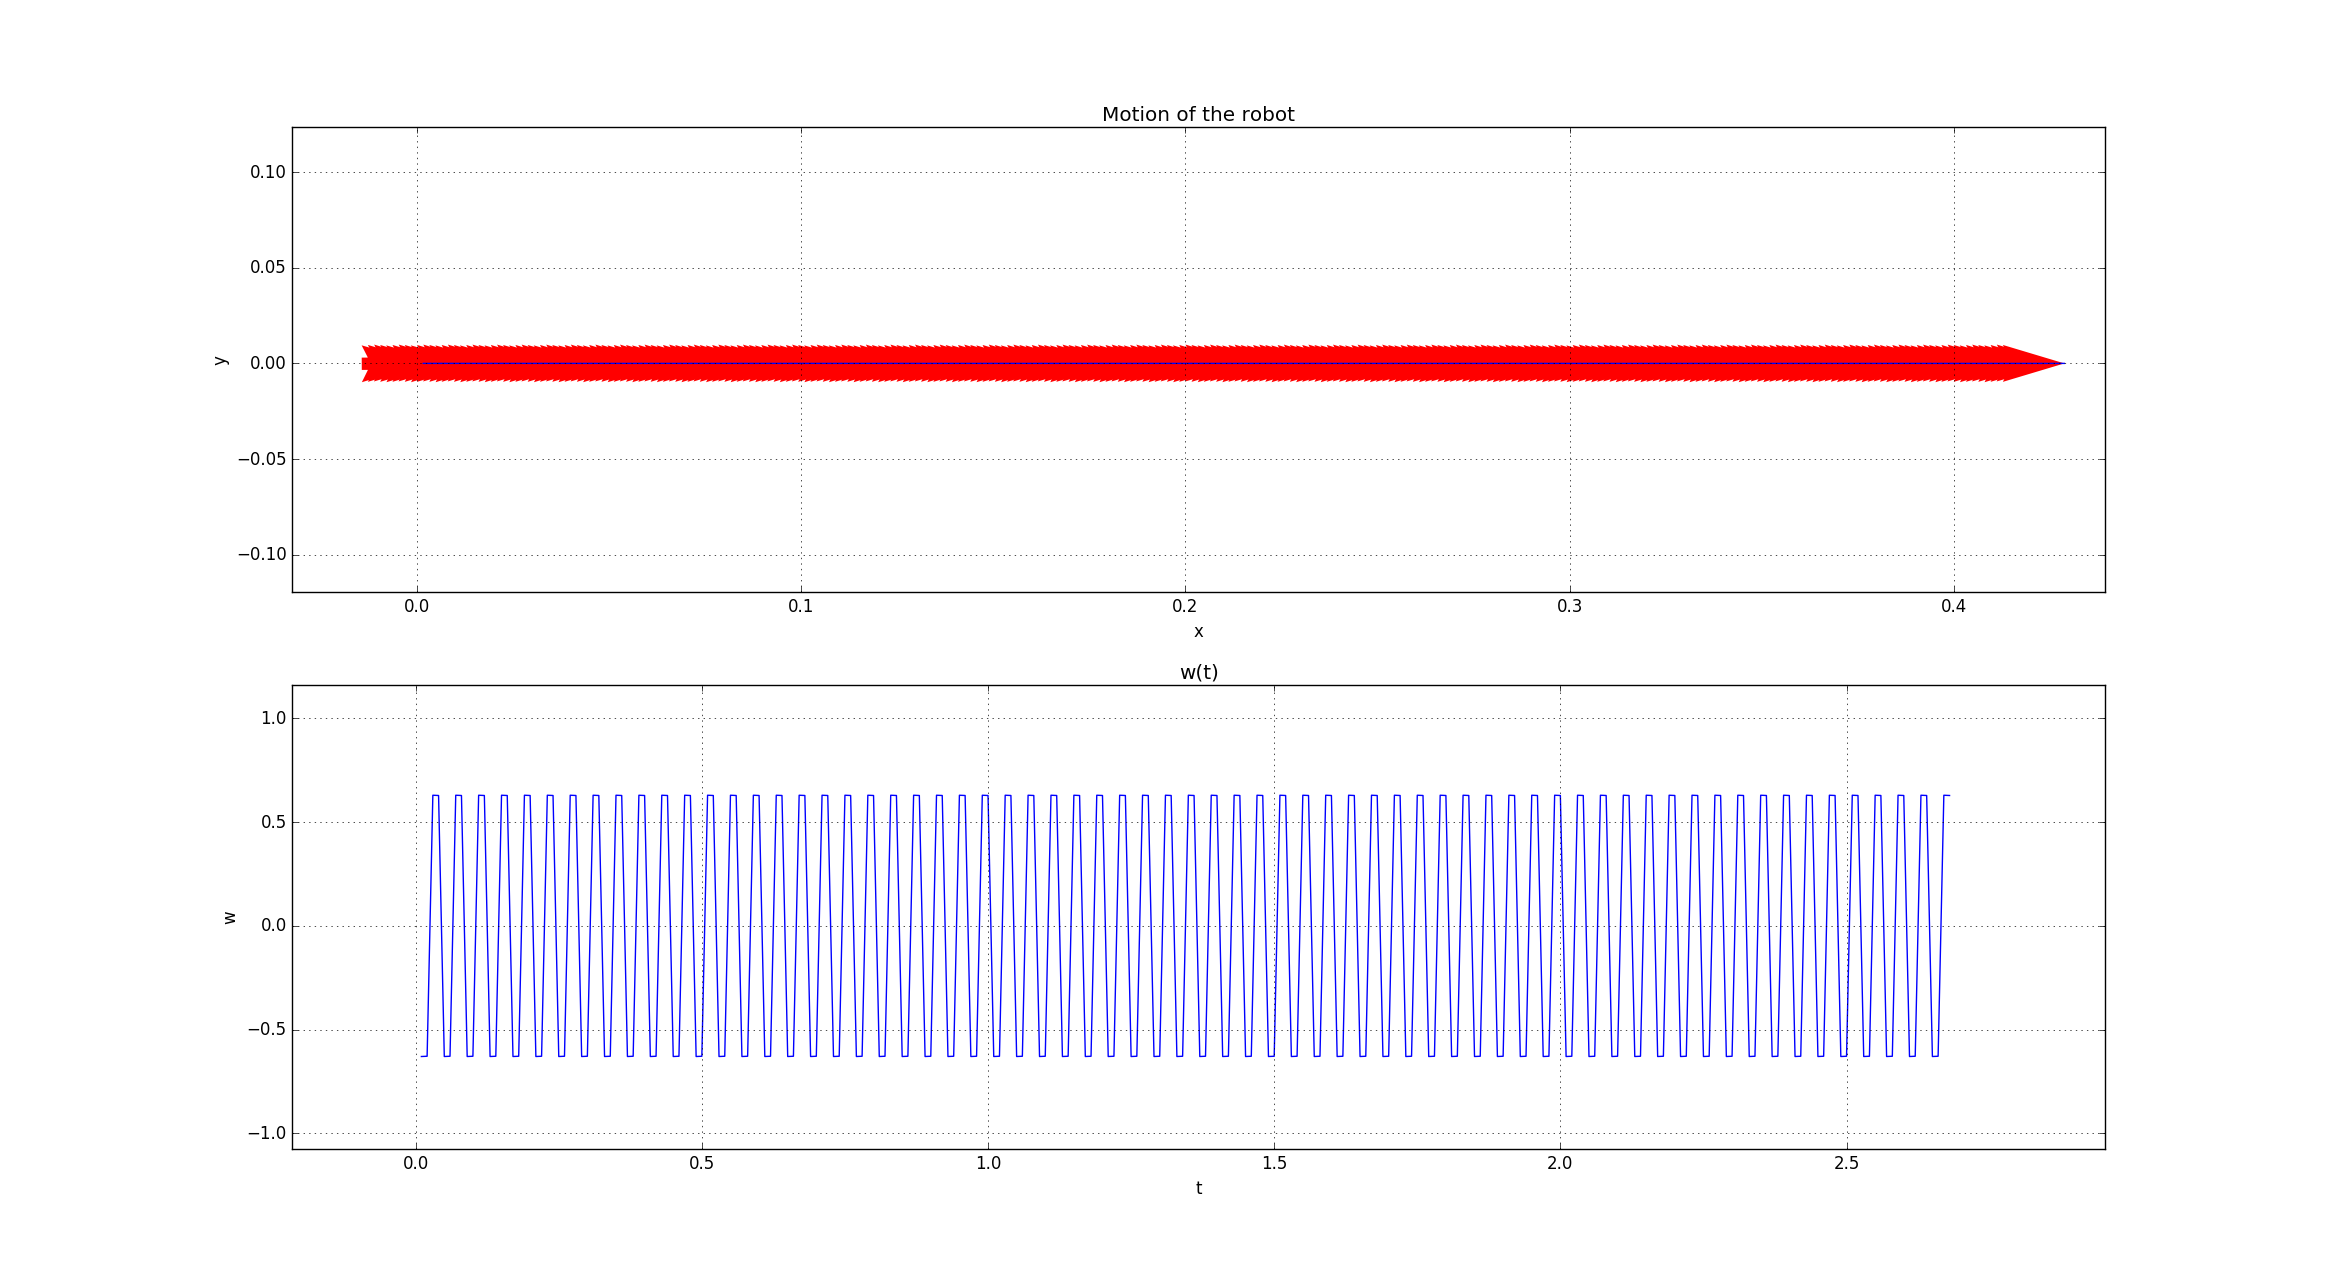
\includegraphics[width=1.9\textwidth]{figs/simulations/critical}
\caption[Simulation: K = 1, Destination (-1, 0)]{(-1, 0) is a destination point that we found out beeing critical. In fact in this case, the point keeps moving straight, without turning and finding the right trajectory. The value of $\omega$ keeps alternating between -1 and 1, but the change is so fast that there are no variations in the actual trajectory.}
\end{figure}

\section{Experiments results}
The following experiments consist of the description of the associated plot, specifying the destination coordinates and the starting ones, taken from the log file generated by the Controller. The gain K is constant to 1 for all the cases we see later. 
\\ The first part of the experiments has been executed with just one destination point given from input and the course is specified in each plot showed below.
\\ These two trials has been executed on a table surface, in order to minimize any errors due to the floor joints.

\begin{figure}[H]
\begin{center}
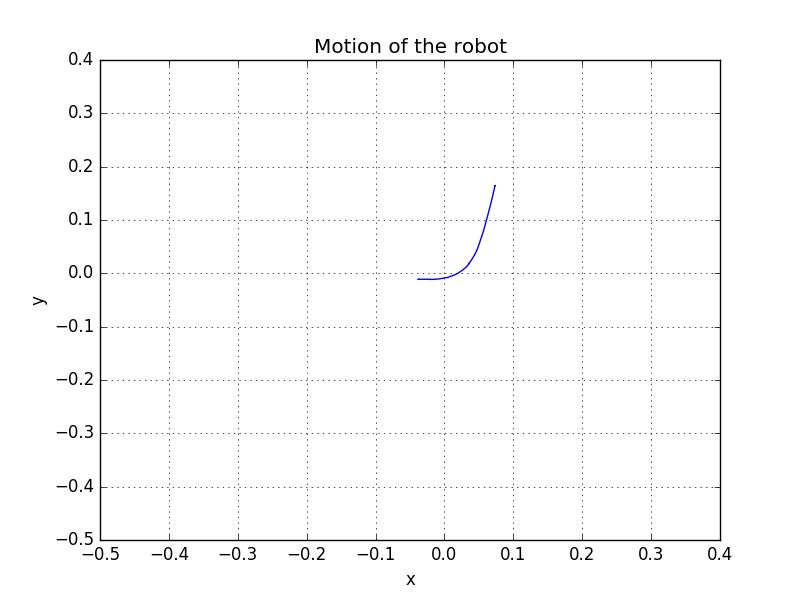
\includegraphics[width=1\textwidth]{figs/experiments/1}
\caption[Experiment: Destination (0.1, 0.3)]{Starting point (-0.0381338653564, -0.0110664644241). Input destination (0.1, 0.3) and the robot reached the point (0.0735064697266, 0.164696762085), with a tolerance of 0.3.}
\end{center}
\end{figure}

\begin{figure}[H]
\begin{center}
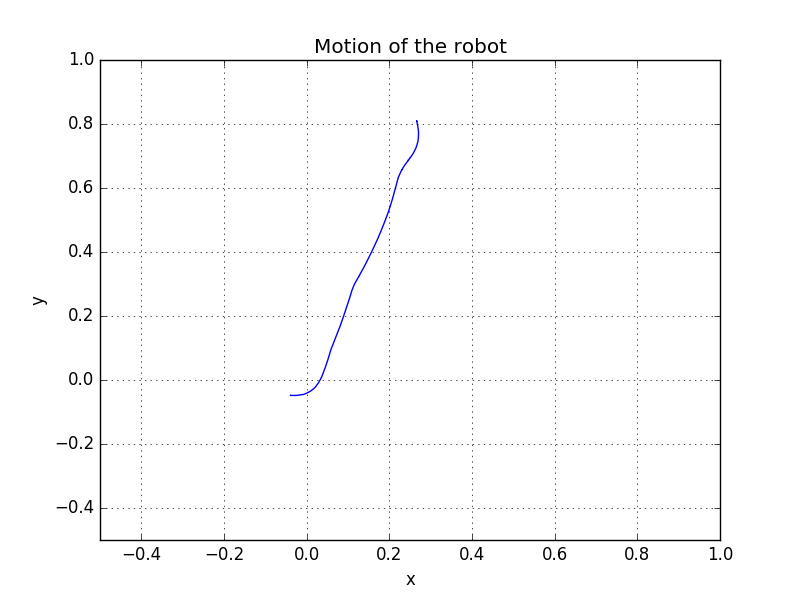
\includegraphics[width=1\textwidth]{figs/experiments/2}
\caption[Experiment: Destination (0.3, 0.9)]{Starting point (-0.0387709541321, -0.0481593437195). The tolerance was decreased to 0.1 and, considering the input destination (0.3, 0.9), the point reached was (0.266358428955, 0.808953735352).}
\end{center}
\end{figure}

The next two experiments has been executed on the floor, in order to have a larger available surface. The tolerance is always constant at 0.1 and the trajectory of the robot is subject to errors introduced by the floor joints.
\begin{figure}[H]
\begin{center}
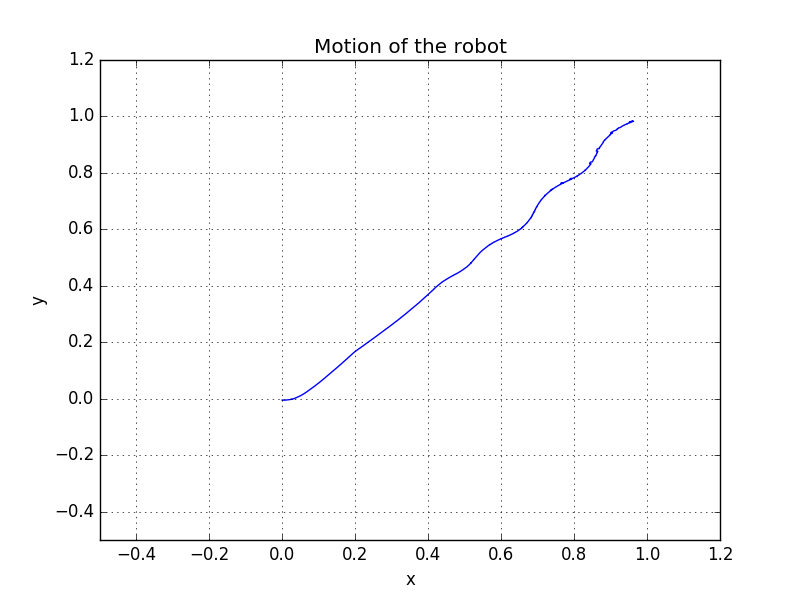
\includegraphics[width=1\textwidth]{figs/experiments/3}
\caption[Experiment: Destination (1, 1)]{Starting point (-0.000775979220867, -0.00463548517227). Input destination (1, 1) and actual reached point (0.958535400391, 0.984300354004).}
\end{center}
\end{figure}

\begin{figure}[H]
\begin{center}
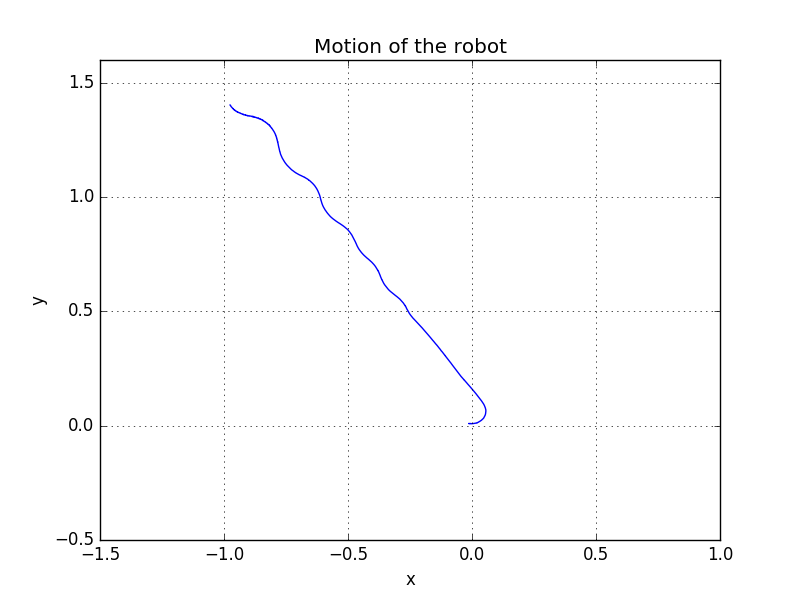
\includegraphics[width=1\textwidth]{figs/experiments/4}
\caption[Experiment: Destination (-1, 1.5)]{Starting point (-0.0120290555954, 0.00933935928345). Input destination (-1, 1.5), so the robot was supposed to be moving to the second quadrant. In fact, the reached point was (-0.975531860352, 1.40306066895).}
\end{center}
\end{figure}

The second part of the experiments consists of keeping the server running while more of one destination point are given from input, in order to make the vehicle travel a square path. The robot is supposed to be moving to the first destination, then stopping and waiting for the next input. Then, it is supposed to be going to the next destination point.
\\ The tolerance is always set to 0.1 for every trial that follows.
\\ These first trials has been executed on the floor, in order to make the robot cover longer distances.

\begin{figure}[H]
\begin{center}
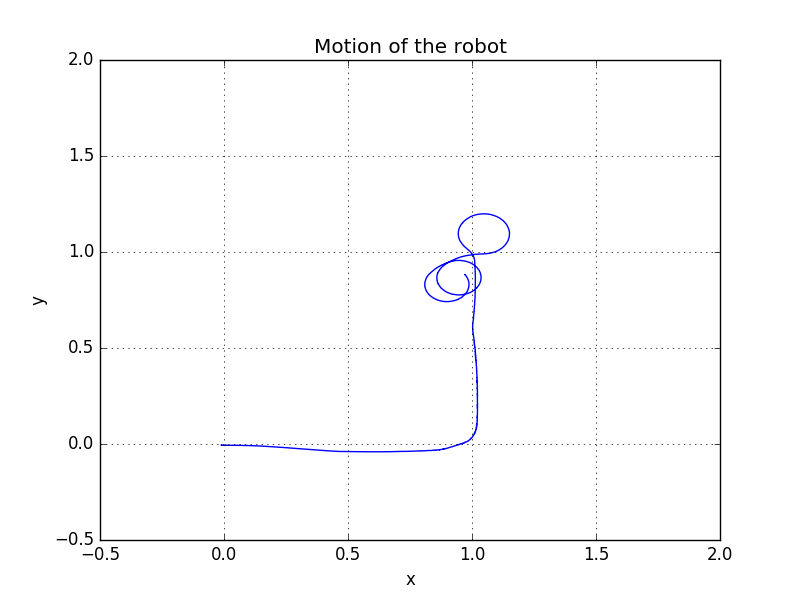
\includegraphics[width=1\textwidth]{figs/experiments/1_1}
\caption[Experiment: Destinations (1, 0), (1, 1), (0, 1)]{Starting point (-0.0111134586334, -0.00597072792053). Input destination (1, 0) and the corresponding reached point (0.903585571289, -0.0204419937134). So, the first motion was successfull. The following input destination was  (1,1), successfully reached in (1.01280255127, 0.901260559082). The following input destination was (0,1) and it was not reached, as it can be seen in the corresponding plot. The vehicle started spinning around itself and then we forced the stop.}
\end{center}
\end{figure}

\begin{figure}[H]
\begin{center}
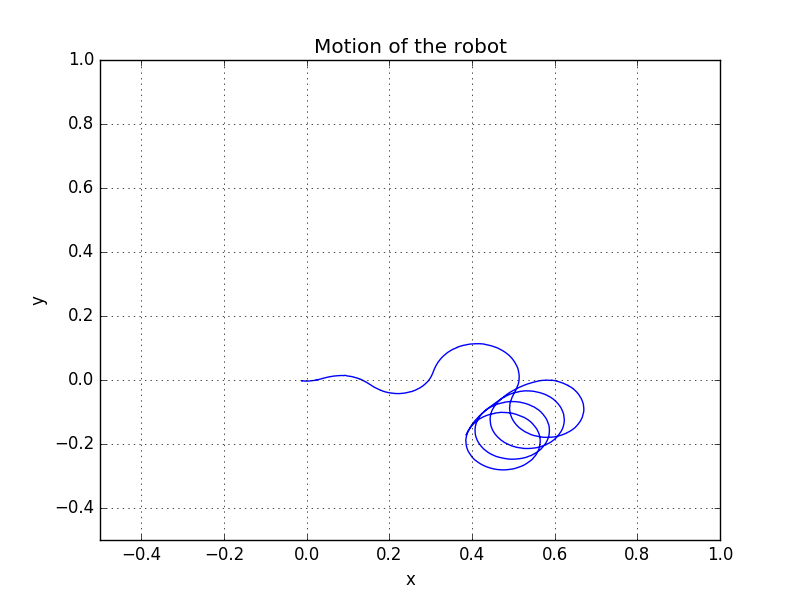
\includegraphics[width=1\textwidth]{figs/experiments/2_1}
\caption[Experiment: Destination (-1, 0)]{Starting point (-0.0122953453064, -0.00266752433777). Input destination (-1, 0), which was not reached. This point was critical even in the simulation phase. The vehicle started spinning around itself, as it can be seen in the plot, without even turning back.}
\end{center}
\end{figure}

\begin{figure}[H]
\begin{center}
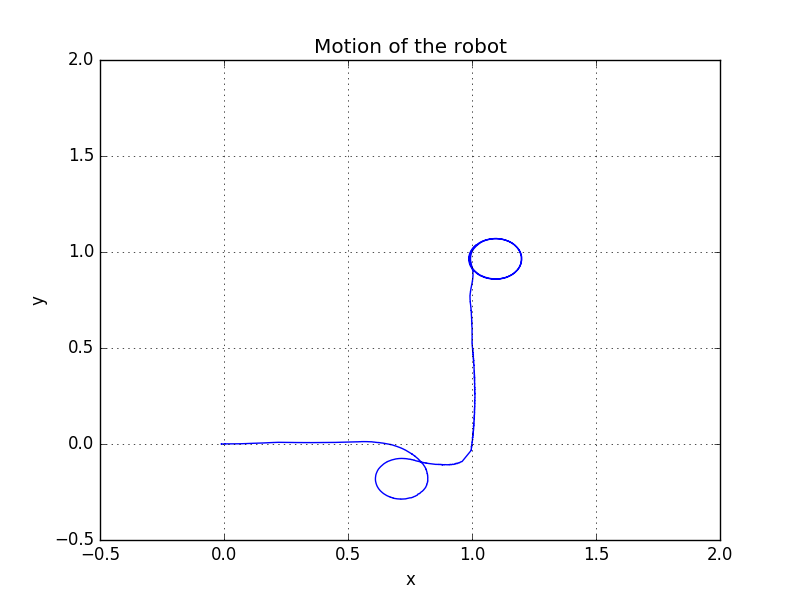
\includegraphics[width=1\textwidth]{figs/experiments/3_1}
\caption[Experiment: Destinations (1, 0), (1, 1), (0, 0)]{Starting point (-0.010465133667, -9.23670381308e-05). Input destination (1, 0), successfully reached in (0.960143249512, -0.0910358200073). Before stopping by the reached point, the robot has made a turn on itself, probably because of the floor joints. The next input destination was (1, 1), successfully reached in (1.00350091553, 0.900240112305). The following input was (0, 0), but it was never reached. The robot started spinning around itself and we forced the stop.}
\end{center}
\end{figure}

The following experiments has been executed on the surface of a table.

\begin{figure}[H]
\begin{center}
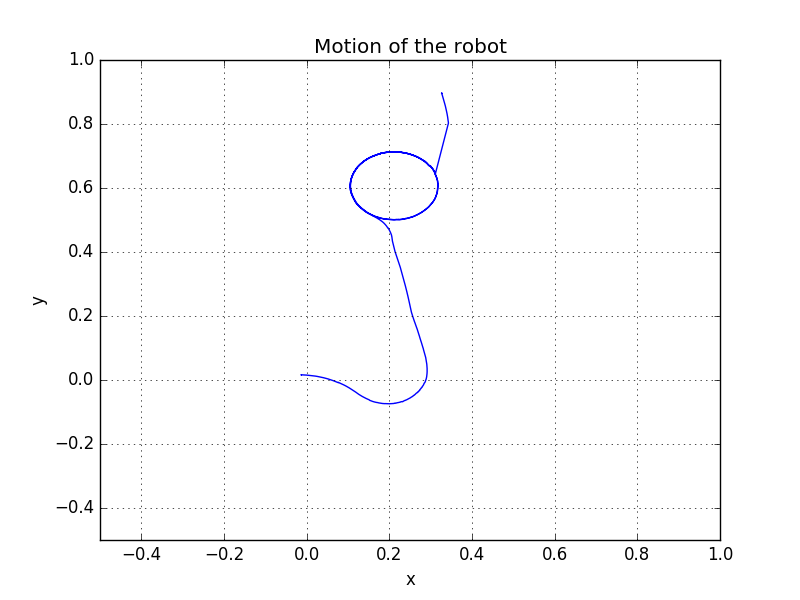
\includegraphics[width=1\textwidth]{figs/experiments/4_1}
\caption[Experiment: Destination (0.2, 0), (0.2, 0.5), (0, 0.5)]{Starting point (-0.013024148941, 0.0162260894775). Input destination (0.2, 0) and the corresponding reached point was (0.103479942322 -0.0250867404938). Successfull movement. The next input destination was (0.2, 0.5), successfully reached in (0.213965026855, 0.400329406738). The following input destination was (0, 0.5). Not reached and forced stop.}
\end{center}
\end{figure}

Until now, we thought that the problem was always the third input destination.

\begin{figure}[H]
\begin{center}
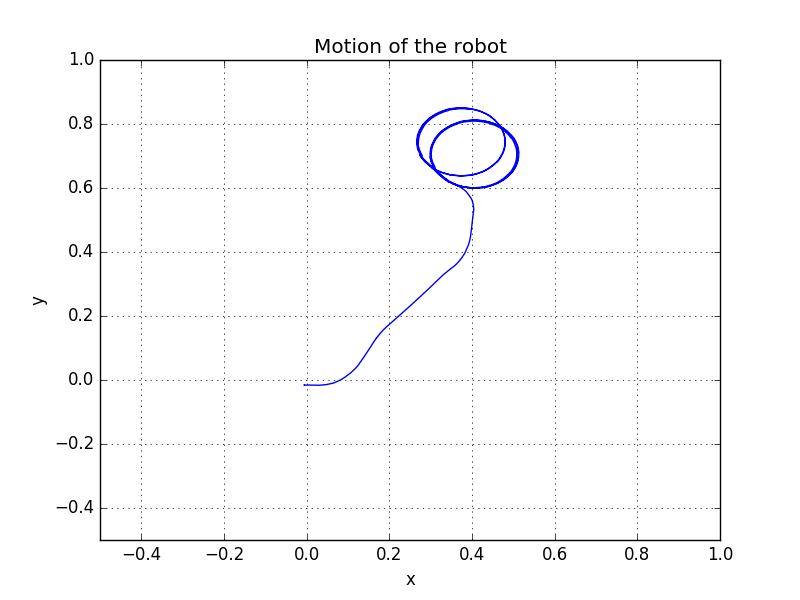
\includegraphics[width=1\textwidth]{figs/experiments/5}
\caption[Experiment: Destination (0.2, 0.2), (0.4, 0.4), (0.4, 0.6), (0.2, 0.6)]{Starting point (-0.00577204990387, -0.015685628891). Input destination (0.2, 0.2), successfully reached in (0.157731643677 0.109515701294). The next input destination was (0.4, 0.4), also successfully reached in (0.329873046875 0.328130767822). The following input destination was (0.4, 0.6) and the corresponding reached point was (0.401092254639, 0.499834869385). The last input destination was (0.2, 0.6), in order to make the robot turn and go back. This did not happen and the vehicle started spinning around itself. We forced the stop.}
\end{center}
\end{figure}

The previous trial has showed that the third input destination was not the problem, since it was reached. So, the issue could be reaching a point behind the robot.
\\ In order to solve this, we tried to make the robot start running in a position different than (0, 0).

\begin{figure}[H]
\begin{center}
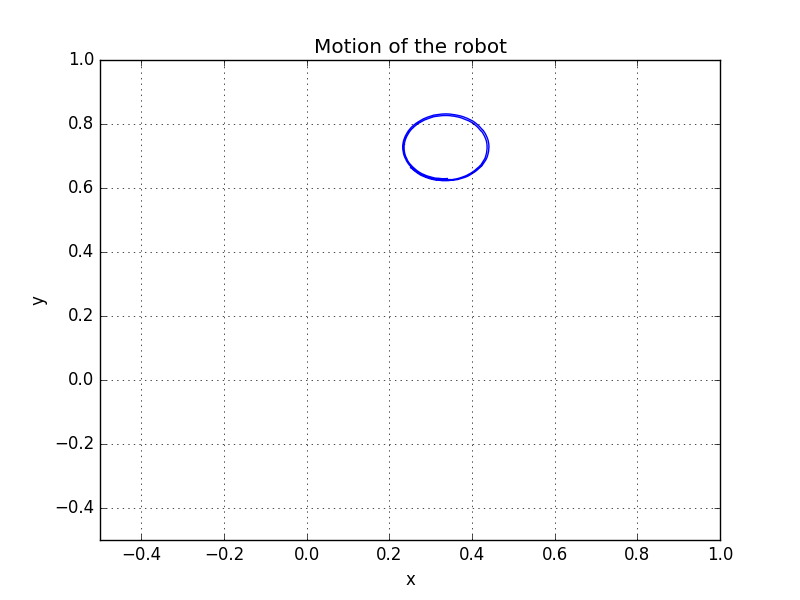
\includegraphics[width=1\textwidth]{figs/experiments/6}
\caption[Experiment: Destination (0, 0)]{Starting point (0.340299926758 0.629281433105). Input destination (0, 0). Not reached and forced stop.}
\end{center}
\end{figure}

In this case the angular speed was constant to -1, so, the issue was still reaching the input point (0,0), which was behind the vehicle.

%%%%%%%%%%%%%%%%%%%%%%%%%%%%%%%%%%%%%

%%%%% SVILUPPI FUTURI %%%%%%
\chapter*{Conclusions} % and future developments}
\addcontentsline{toc}{chapter}{Conclusions} %  and future developments}
%%%%%%%%%%%%%%%%%%%%%%%%%%
As we know, the mobile robot trajectory is a continuos vector function in time domain. It is made up by $m$ scalar functions, as many as are system controls (e.g., in our case linear speed and angular speed). Another trajectory definiton is course, to which is associated a temporal law through which the path is followed by the robot. We have used this concept by classifying it according to the task assigned to the robot: point to point control problem. The robot under exam has to arrive to a final position from a starting position. For a point to point problem, it is sufficient to solve the problem in a direct way, by calculating motion law. In this way, the course turns out to be an output of the planning algorithm. From the point of view of the control, the problem is to stabilize the robot in a point of equilibrium in the space of the configuration variables. For the stabilization, we have used the closed loop control, using a feedback law named continuos status feedback.
The features of controllability and the system constraints change as the model we are working with varies. In our case, we have considered appropriate to put a bound on the angular speed in order not to destabilize the system. As we said, the bound depends on the model, so we have set it at [-1, 1] in order not to make unstable the system by going into saturation. We can obtain the same result by limiting the gain to a value that is not too high, because this one could bring about having a dangerous increase of the angular speed, which means a possible instability of the system.
The solution has been using a feedback control of the estimated error in order to obtain a certain degree of robustness of the overall control.
% %%%% APPENDIX %%%%%
% \appendix
% \chapter{Appendix title}
% %%%%%%%%%%%%%%%%%%%%

%%%%%%%%%% BIBLIOGRAPHY %%%%%%%%%%%%%%
\bibliography{bibliography}
\bibliographystyle{plain}
\addcontentsline{toc}{chapter}{Bibliography}
%%%%%%%%%%%%%%%%%%%%%%%%%%%%%%%%%%%%%%

\end{document}
